% SciForge: A Multimodal Research-Native AI Workbench for Scientific Discovery
% Technical Report Outline

\documentclass[sn-basic,Numbered,pdflatex]{sn-jnl}
\ifdefined\pdfminorversion\pdfminorversion=7\fi

% === Packages ===
\usepackage{graphicx}
\usepackage{float}
\usepackage{multirow}
\usepackage{amsmath,amssymb,amsfonts}
\usepackage{amsthm}
\usepackage{mathrsfs}
\usepackage[title]{appendix}
\usepackage[table]{xcolor}
\usepackage{textcomp}
\usepackage{manyfoot}
\usepackage{tikz}
\usetikzlibrary{positioning}
\usepackage{forest}
\usepackage{booktabs}
\usepackage{array}
\usepackage{xurl}
\usepackage{microtype}
\usepackage{placeins}
\usepackage{hyperref}

% Keep figure/caption rhythm compact without crowding the surrounding prose.
\setlength{\textfloatsep}{13pt plus 3pt minus 2pt}
\setlength{\floatsep}{13pt plus 3pt minus 2pt}
\setlength{\intextsep}{13pt plus 3pt minus 2pt}
\setlength{\dbltextfloatsep}{13pt plus 3pt minus 2pt}
\setlength{\dblfloatsep}{13pt plus 3pt minus 2pt}

\newcommand{\cmark}{\ensuremath{\checkmark}}
\newcolumntype{L}[1]{>{\raggedright\arraybackslash}p{#1}}
\newcolumntype{C}[1]{>{\centering\arraybackslash}p{#1}}

% === Metadata ===
\title[SciForge: Multimodal Research-Native AI Workbench]{SciForge: A Multimodal Research-Native AI Workbench for Scientific Discovery}

\author*[1]{\fnm{Author} \sur{Names}}\email{author@example.com}

\affil*[1]{\orgdiv{Institute}, \orgname{University}, \orgaddress{\city{City}, \country{Country}}}

% === Abstract keywords ===
\abstract{
Scientific work increasingly spans heterogeneous artifacts---papers, code, datasets, scientific file formats, model outputs, figures, manuscripts, and team decisions---yet general-purpose AI assistants rarely preserve these objects as a coherent, auditable research state. We present SciForge, a multimodal research-native AI workbench that reserves the graphical interface for human judgment while search, parsing, model routing, workflow execution, plotting, writing, and presentation generation run as modular agent-accessible services. SciForge is built around five pillars: (i) \emph{goal-scoped scientific decision governance} for \textbf{goal-oriented} research, with review gates and shared review surfaces; (ii) \emph{translate-then-reason} for \textbf{multimodal} input, routing scientific objects through domain translators before the agent reasons; (iii) \emph{evidence governance} for \textbf{auditable} traceability, linking claims to provenance chains and audit findings; (iv) \emph{collaborative team science} for \textbf{collaborative} research, enabling multi-role decision governance, with shared team workspaces planned for future releases; and (v) \emph{real-world application scenarios} for \textbf{practical} impact, integrating end-to-end scientific workflows including BGC discovery, protein structure prediction, automated figure generation, and multi-format document parsing. The system combines a thin interaction layer, contextual research capability patterns, an Agent Runtime and Workflow Engine, an Evidence-DAG audit sidecar, a Scientific Model Router, and local scientific memory backed by reusable worker services. SciForge currently runs as a desktop application, with mobile supervision support; future releases will deepen team collaboration through shared review surfaces and decision governance. The system is open-source and available at \url{https://github.com/AGI4Sci/SciForge}.
}

\keywords{SciForge, AI workbench, scientific discovery, agentic workflow, evidence-aware AI, multimodal science, research automation}

%% === BEGIN DOCUMENT ===
\begin{document}

\maketitle

\vspace{-12pt}
% ============================================================
\section{Introduction}
% ============================================================

\subsection{Background and Motivation}

Scientific discovery is becoming increasingly computational, multimodal, and collaborative. A single research project may move among scholarly papers, experimental protocols, command-line tools, notebooks, gene and variant files, protein sequences, three-dimensional structures, molecular records, single-cell matrices, generated figures, manuscript drafts, slide decks, and group decisions. These objects are not independent files. A manuscript claim may depend on a raw dataset, a preprocessing script, a model run, a visualization parameter, a literature passage, and a later human decision about whether the evidence is strong enough to use. As a result, the central bottleneck is no longer only access to models or tools, but the lack of a persistent environment that can organize scientific objects, agent actions, human decisions, and evidence traces as one coherent research state.

Recent AI systems have demonstrated impressive capabilities for literature search, hypothesis generation, coding, experimentation, and scientific writing \cite{futureHousePlatform2025,googleCoScientist2025,sakanaAIScientist2024,agentLaboratory2025,paperQA2024}. At the same time, desktop and terminal-capable scientific workbenches show the importance of keeping execution close to local files, remote servers, and HPC environments \cite{anthropicClaudeScience2026,omicOSOverview2026,omicsClaw2026,operonGitHub2026,claudePrism2026}. However, most existing systems still emphasize either task-specific intelligence, conversational assistance, or local execution surfaces. They rarely treat the full research process as a \textbf{goal-oriented}, \textbf{multimodal}, \textbf{auditable}, and \textbf{collaborative} workflow in which scientific data, agent reasoning, generated artifacts, and manuscript claims remain connected over time.

This gap matters because scientific AI agents must satisfy four demands that are absent from general-purpose assistants. First, \textbf{goal-oriented} research design is indispensable: scientific work is goal-scoped, not session-scoped—researchers need persistent objectives, review gates, and shared decision records that span turns, tools, and collaborators. Second, \textbf{multimodal} inputs are the norm: scientific files arrive in native representations poorly suited to direct prompting, including FASTA sequences, PDB or mmCIF structures, SMILES strings, variant files, and cell-omics tables. Third, \textbf{auditable} evidence is non-negotiable: researchers need to know which data, script, model, parameter, paper, or expert translation supported a conclusion; whether a figure matches the claim it is used to support; and when a proposed action requires human or principal-investigator approval. Fourth, \textbf{collaborative} governance is essential: scientific work involves team decisions, goal-scoped approvals, cross-session handoffs, and shared review of claims and evidence. A stateless chat transcript addresses none of these demands.

We present \emph{SciForge}, a multimodal research-native AI workbench for scientific discovery. SciForge is designed as a local-first operating environment for research rather than a wrapper around a single model. Its architecture organizes interaction surfaces, research capability patterns, a core engine with evidence governance, a scientific model router, and local-first infrastructure into a coherent layered workbench; Section~\ref{sec:system-architecture} describes each layer in detail.

\subsection{Contributions}

SciForge's core scientific contribution is organized around five pillars, each addressing a distinct gap in current research AI systems:
\begin{itemize}
    \item \textbf{Native scientific object processing with translate-then-reason:} end-to-end file ingress exposes four classes---protein sequences (.faa; .fasta/.fa with per-record conservative content classification), protein structures (.pdb/.cif/.mmcif), molecules (.smi/.smiles), and single-cell transcriptomics (via Cell2Sentence (C2S))---routed through domain-expert translators (Esm2Text~\cite{abdine2023prot2text}, Prot2Text~\cite{abdine2023prot2text}, BioT5~\cite{pei2024biot5}, and C2S~\cite{rizvi2025c2s}) that return structured expert observations before the main agent reasons. The translator output is an evidence candidate, not a verified scientific fact; the human remains responsible for judgment.

    \item \textbf{Artifact- and run-grounded evidence governance:} every agent action---file read, model call, tool invocation, script execution---can attach structured provenance (software version, parameters, environment, random seed) to a thread-level Evidence Snapshot. Users designate when to commit a snapshot, marking which evidence supports which claim. A read-only audit sidecar inspects these snapshots and surfaces potential gaps without blocking the agent's work.

    \item \textbf{Goal-scoped scientific decision governance:} a Project DAG organizes research goals, evidence snapshots, and review decisions into a shared, auditable structure. Researchers can inspect evidence chains, record review decisions, set goal-level execution policies (autonomous, checkpointed, or supervised), and promote artifacts through candidate and certified release gates.

    \item \textbf{Collaborative team science:} SciForge supports multi-role decision governance with reviewer/approver roles and IM-based coordination channels (Zulip, Discord, WeChat, Feishu) for remote task submission and status supervision. The Project DAG enables collaborative review workflows where researchers inspect Evidence Snapshots, record ReviewItems with role-attributed decisions, and advance artifacts through candidate/certified release gates. Shared team workspaces with cross-session research memory synchronization are planned for a future release.

    \item \textbf{Real-world scientific application scenarios:} SciForge integrates end-to-end scientific workflows for several concrete research tasks, including biosynthetic gene cluster (BGC) discovery from genomic data, protein structure prediction and analysis via AlphaFold3 integration, automated scientific figure generation with journal-style rendering, multi-format document parsing for scientific literature ingestion, and AI-assisted presentation slide deck generation from research artifacts. These applications demonstrate the system's ability to bridge the gap between general-purpose AI assistance and domain-specific scientific practice.
\end{itemize}

SciForge treats each scientific interaction---literature triage, hypothesis refinement, manuscript drafting, artifact inspection, and presentation---as a first-class research task with explicit evidence trails, audit findings, and governance checkpoints. The SciForge codebase, including the Evidence-DAG audit worker, decision-record contracts, agentic skills, and scientific model router, is open source at \url{https://github.com/AGI4Sci/SciForge}.

\section{Related Work}
% ============================================================

\subsection{GUI-Based Scientific Workbenches}

GUI-based scientific workbenches, including desktop and web applications, make AI assistance accessible through human-facing workspaces. Claude Science is the closest broad commercial reference: it is described as an AI workbench for scientists with desktop, local, SSH, and HPC-facing execution, scientific skills, specialist agents, generated artifacts, and reviewer agents for citations and calculations \cite{anthropicClaudeScience2026}. ClaudePrism focuses on the manuscript side of the workflow, combining a native desktop environment with local LaTeX compilation, Python environments, Claude Code sessions, and scientific writing skills \cite{claudePrism2026}. Web tools such as Elicit and Consensus provide polished interfaces for literature search, synthesis, and research-agent style review \cite{elicit2026,consensus2026}. These systems demonstrate the importance of usable research interfaces, but they are usually centered on one model family, one workflow domain, or one user session. SciForge instead treats the GUI as a thin layer for human judgment over a local, modular, multi-agent research substrate.

\subsection{Terminal Workbenches}

Terminal-oriented workbenches prioritize execution close to local files, remote servers, and HPC environments. OmicOS provides a Rust \texttt{omicos-core} binary that can run as a local daemon serving a browser UI or as \texttt{omicos cli}, with analysis code running in a shared IPython kernel and raw data remaining local \cite{omicOSOverview2026,omicOSServe2026,omicOSCLI2026}. OmicsClaw follows a local-first multi-omics design with CLI, TUI, desktop, web backend, and SSH remote execution surfaces over a shared agent loop \cite{omicsClaw2026}. Operon targets bioinformatics workflows across desktop and remote cluster environments, using persistent terminal sessions so jobs execute where data and schedulers live \cite{operonGitHub2026}. These systems are strong at local and remote execution, but they generally expose tools and workflows rather than a unified layer for multimodal scientific routing, research decision surfaces, team supervision, and manuscript-to-artifact continuity.

\subsection{API and Research Agents}

API-based and research-prototype agents explore more autonomous scientific reasoning. FutureHouse exposes agents for literature search, deep review, precedent search, and chemistry planning through a web/API platform \cite{futureHousePlatform2025}. Google's AI Co-Scientist studies multi-agent hypothesis generation, debate, and ranking for biomedical research \cite{googleCoScientist2025}. The AI Scientist and Agent Laboratory automate parts of the machine-learning research loop, including ideation, coding, experimentation, paper drafting, and review \cite{sakanaAIScientist2024,agentLaboratory2025}. Literature systems such as PaperQA2, OpenScholar, and ScholarQA focus on retrieval-augmented scientific question answering and literature synthesis \cite{paperQA2024,openScholar2024,scholarQA2025}. These systems demonstrate the power of specialized agents, but they are less focused on being a persistent local workbench where data, code, figures, decisions, and generated artifacts remain in one workspace.

\subsection{Comparison and Positioning}

While each of the three system categories addresses a distinct facet of the AI-assisted research life cycle, SciForge is designed to unify them within a single workbench. The comparison spans five key dimensions: execution, model governance, evidence quality, research continuity, and goal-oriented research design.

\textbf{Execution architecture.} GUI workbenches such as Claude Science and ClaudePrism deliver polished interactive experiences but are typically constrained to one model provider and one local session. Terminal workbenches---OmicOS with its hybrid daemon plus browser model, OmicsClaw with multi-surface CLIs, and Operon with persistent terminal sessions---excel at running code where data and schedulers reside, yet they expose tools and pipelines rather than a unified research workbench. SciForge bridges these worlds by providing a GUI for human judgment while keeping a local-first workspace where execution can span desktop, SSH, and HPC environments.

\textbf{Model governance.} The reviewed public materials commonly emphasize a single provider family or manual switching between separate tools. SciForge's Scientific Model Router combines multi-provider routing with a deliberately narrow translate-then-reason file-ingress path covering four modality classes: protein sequences (Esm2Text~\cite{abdine2023prot2text}), protein structures (Prot2Text~\cite{abdine2023prot2text}), molecules (BioT5~\cite{pei2024biot5}), and single-cell transcriptomics (Cell2Sentence~\cite{rizvi2025c2s}); unsupported formats fail closed. Literature is handled through search, PDF anchoring, and source attribution, not as a scientific modality translator. We did not find this same integrated combination documented as a first-class feature in the reviewed categories.

\textbf{Evidence quality and governance.} Research agents such as FutureHouse, AI Co-Scientist, and the AI Scientist produce outputs from variable-quality evidence; in the publicly documented materials we reviewed, we did not observe the same integrated combination of claim--evidence audit trail, PROV-JSON provenance, and quality gates in a single research workbench. SciForge threads claims through an Evidence DAG backed by PROV-JSON provenance, audit runs, risk digests, and explicit quality gates. This governance layer is designed to make agent outputs inspectable and auditable.

\textbf{Research continuity.} Many reviewed systems foreground per-session interaction. SciForge maintains goal-centered research memory as scoped free-text records (scope, tags, confidence, timestamps, context) across sessions; typed goals and decision events belong to the Project DAG, enabling long-running multi-session scientific workflows rather than only single-turn conversations. The combination of research memory, workflow engine, and evidence governance creates a persistent research workspace whose integrated design---tying thread-level Evidence Snapshots to goal-scoped Project Snapshots with audit and release semantics---we did not find documented as a first-class, integrated feature in the public materials of the reviewed GUI, terminal, and API-agent systems.

\textbf{Goal-oriented research design.} SciForge anchors every thread and project to an explicit goal scope with defined review gates, decision records, and release semantics. This design ensures that scientific objectives are persistent, auditable, and governable across multiple turns, tools, and contributors.

Table~\ref{tab:terminal_related_work} summarizes these differences at the category level, while the detailed capability differentiation in Appendix~\ref{tab:capability_differentiation} provides a feature-level comparison against common approaches.

\begin{table}[ht!]
\caption{High-level comparison of scientific AI system categories. A checkmark indicates first-class or documented support as a primary design goal in the publicly reviewed materials. Absence of a checkmark does not prove absence of a feature; it indicates we did not find documented first-class support in the reviewed materials. $\dagger$~Planned for a future release.}
\label{tab:terminal_related_work}
\scriptsize
\centering
\setlength{\tabcolsep}{4pt}
\renewcommand{\arraystretch}{1.15}
\begin{tabular}{@{}L{5.0cm} C{1.30cm} C{1.30cm} C{1.30cm} C{1.30cm}@{}}
\toprule
\textbf{Capability} &
\textbf{\shortstack{GUI\\WB}} &
\textbf{\shortstack{Terminal\\WB}} &
\textbf{\shortstack{API\\agent}} &
\textbf{SciForge} \\
\midrule
Human Interface --- GUI for interactive research & \cmark &  &  & \cmark \\
Local Execution --- local/HPC compute, local-first data &  & \cmark &  & \cmark \\
Sci. Tools --- fail-closed native format ingestion &  &  &  & \cmark \\
Sci. Multimodal Routing --- enhanced scientific multimodal understanding &  &  &  & \cmark \\
Workflow Automation --- DAG-based scheduled protocols &  &  &  & \cmark \\
Research Memory --- cross-session knowledge persistence &  &  &  & \cmark \\
Evidence Governance --- provenance, audit trail, release gates &  &  &  & \cmark \\
Team Workspace --- multi-user collaboration\textsuperscript{$\dagger$} &  &  &  & \textsuperscript{$\dagger$} \\
\bottomrule
\end{tabular}
\end{table}

SciForge combines these categories rather than competing with only one of them. It keeps the usability of GUI workbenches, the locality and composability of terminal systems, and the task power of scientific agents, while adding fail-closed scientific-object handling, content-addressed artifacts with structured selection and provenance, specialist domain translation, run-grounded evidence governance with immutable snapshots and an audit sidecar, and goal-scoped decision governance with explicit release semantics.

% ============================================================
\section{System Architecture}\label{sec:system-architecture}
% ============================================================

\subsection{Overall Design Philosophy}

SciForge is organized as a layered research operating environment. \textbf{Layer~1} provides thin judgment surfaces for desktop, group, and mobile interaction. \textbf{Layer~2} encapsulates six research capability patterns---Literature Review, Idea Generation, Experiment Design, Experiment Execution, Analysis \& Iteration, and Scientific Communication---that cover the scientific workflow while sharing one evidence-aware control chain. \textbf{Layer~3} houses the core engine: agent runtime, workflow automation, scoped memory, and evidence governance. \textbf{Layer~4} is the Scientific Model Router that detects modality and dispatches to domain-expert translators. \textbf{Layer~5} supplies infrastructure: local memory, modular workers, scientific connectors, and reproducible run substrate.

SciForge follows three implementation principles that distinguish it from feature-heavy desktop software:

\begin{enumerate}
    \item \textbf{Thin GUI.} The interface appears only when human judgment is needed---reviewing, annotating, approving, comparing; all other capabilities run in the background agent runtime.
    \item \textbf{Modular services.} Search, parsing, plotting, model routing, workflow execution, and presentation generation run as MCP-compatible tools or worker processes, keeping the application close to a thin interaction shell \cite{anthropicMCP2024}.
    \item \textbf{Local-first evidence model.} Data, traces, artifacts, and evidence graphs remain anchored to the research workspace; remote collaboration and mobile access are control channels, not replacements for local state.
\end{enumerate}

Figure~\ref{fig:sciforge_framework} summarizes the layered architecture.

\FloatBarrier
\begin{figure*}[ht!]
    \centering
    
\includegraphics[width=0.98\textwidth,height=0.86\textheight,keepaspectratio]{figures/SciForge_Framework_v3.pdf}
    \caption{SciForge system framework. Layer~2 exposes six scientific-workflow capabilities---Literature Review, Idea Generation, Experiment Design, Experiment Execution, Analysis \& Iteration, and Scientific Communication. Each capability enters the same evidence-aware control chain---ingress, translation, execution, evidence capture, audit, and release---built on the interaction surfaces, core engine, scientific model router, and local-first infrastructure.}
    \label{fig:sciforge_framework}
\end{figure*}

\subsection{User Interaction and Collaboration (Layer~1)}
Layer~1 exposes three interaction surfaces driven by the same underlying runtime. The \textbf{desktop application} provides a thin GUI reserved for human judgment---reviewing evidence, annotating figures, comparing candidate artifacts, and approving release decisions---while execution runs in the background. \textbf{Group chat integration} (Zulip, Discord, WeChat, Feishu) enables remote task submission, status polling, and lightweight approvals without switching context. \textbf{Mobile supervision} enables remote monitoring and intervention for long-running experiments, with task submission and review actions gated through the same governance model.

\subsection{Research Capability Patterns (Layer~2)}
SciForge supports six research capability patterns with explicit scientific input--output boundaries. \emph{Literature Review} maps papers and source records to a field map that summarizes prior work and the current state of a domain. \emph{Idea Generation} maps existing evidence to research questions, hypotheses, and candidate methods. \emph{Experiment Design} turns a selected idea into a test plan with validation procedures, metrics, controls, and success criteria. \emph{Experiment Execution} maps that plan to run records and artifacts by executing code, conducting experiments, invoking instruments, or delegating to computational pipelines. \emph{Analysis \& Iteration} maps results to diagnoses, revised assumptions, and a justified next step. \emph{Scientific Communication} maps reviewed evidence and research artifacts to papers, reports, figures, and presentations. These capability patterns cover a common scientific workflow but are not a rigid linear pipeline: researchers may enter at any stage and iterate between stages. They remain contextual patterns within one workbench rather than independent applications with separate execution semantics. Regardless of entry point, each task follows the same evidence-aware control chain: (1) task and object ingress; (2) fail-closed translation when a native scientific object requires a domain expert; (3) delegated agent and worker execution through Layers~3 and~4; (4) provenance-attached evidence candidates with artifact and run lineage; (5) a thread-scoped Evidence Snapshot and advisory audit; and (6) goal-scoped review and candidate/certified release through the Project DAG and human PI.

\subsection{Core Engine (Layer~3)}
The Core Engine plans and executes research work through coordinated subsystems.

SciForge uses two connected evidence layers for scientific governance. The \textbf{Evidence DAG} (thread-scoped) automatically constructs a claim--source--reasoning graph from each agent session's completed turns and persists the graph as PROV-JSON. The \textbf{Project DAG} (goal-scoped) consumes immutable Evidence DAG snapshots across sessions, merges equivalent findings while preserving independent source paths, and links claims to project objectives. Both layers compile asynchronously behind the main agent, keeping evidence up to date without blocking exploration. Audit runs are read-only sidechains that produce structured risk digests---flagging ungrounded claims, unresolved contradictions, weak support, or low-credibility sources---without mutating DAG state. All decisions, whether human or AI, enter through structured Decision Events, giving every modification a traceable, reviewable record.

The \textbf{Agent Runtime} uniformly supports multiple agent backends---Codex, Claude Code, and custom runtimes---allowing research groups to select the execution environment that best matches their scenario: Codex for local-first interactive coding with full workspace access, Claude Code for extended autonomous task chains, and custom runtimes for specialized scientific computing or institutional deployment requirements. Across all backends, the Runtime coordinates the main agent, delegated sub-agents, tool execution, workspace operations, MCP worker invocation, and long-running task recovery through a consistent API surface. The \textbf{Workflow Engine} formalizes reusable pipelines with code, agent, tool, and approval nodes; scheduled execution and loop-style fixed protocol automation are treated as run modes rather than separate architectural modules. \textbf{Scoped Research Memory} stores free-text records (scope, tags, confidence, timestamps, context) across sessions; typed goals and decision events belong to the Project DAG. \textbf{Evidence \& Release Governance} exposes goal-scoped release decisions (candidate and certified gates) through the Project DAG without synchronously blocking exploratory execution.


\subsection{Scientific Model Router (Layer~4)}
The \textbf{Scientific Model Router} is a core architectural innovation of SciForge, acting as a universal model invocation plane that abstracts away provider heterogeneity while retaining the full expressiveness of each backend. Rather than forcing a lowest-common-denominator interface, the Router supports three request--response protocols---OpenAI Chat Completions, OpenAI Responses, and Anthropic Messages---selected per provider through a normalized endpoint format, allowing each model to be invoked through its native, most capable API surface.

\textbf{Intelligent Auto-Routing.} The Router includes a lightweight classifier that inspects the user request and recent context to automatically select the appropriate reasoning effort (off, high, or max), with a deterministic heuristic fallback so routing decisions do not rely on a single point of failure.

\textbf{Provider-Aware Optimization.} For DeepSeek models, the Router performs proactive reachability probing, applies native thinking controls, and computes real-time cache-aware cost estimation in both USD and CNY. For all providers, it implements automatic retry with backoff, error classification, and stream-idle timeout detection.

\textbf{Output Robustness and Repair.} The Router repairs malformed tool-call arguments---stripping Markdown fences and recovering partial JSON---and extracts embedded images from tool results as standard model attachments, enabling multimodal reasoning chains across scientific visualizations and model analysis.

\textbf{Scientific Modality Routing.} For scientific files, the Router detects modality-specific extensions and applies one of two handling paths. \emph{Translate-then-reason} applies to four currently supported modalities: protein (.faa; .fasta/.fa with per-record conservative content classification) translated by Esm2Text, protein structures (.pdb, .cif, .mmcif) by Prot2Text, small molecules (.smi, .smiles) by BioT5, and single-cell transcriptomics via Cell2Sentence (C2S). Each translator output carries provenance metadata, allowing the main agent to reason over structured expert observations. VCF, BED, GFF, and MGF are unsupported and fail closed; raw content is not routed to the general reasoner.

Multimodal translation caches store scientific and visual observations by content hash, enabling repeated requests to reuse expert evidence without recomputing final conclusions.


\subsection{Infrastructure (Layer~5)}
The Infrastructure layer provides the durable substrate that anchors research activity to the local workspace. \textbf{Local Scientific Memory} stores papers, datasets, parsed documents, scientific file manifests, embeddings, indexes, tool outputs, run metadata, and artifact caches. The \textbf{Modular Capability System} packages computational functionality as Skills, MCP servers, Plugins, HTTP services, or worker processes---each independently versioned and upgradeable. \textbf{Scientific Connectors} normalize external resources such as papers, datasets, databases, APIs, instruments, notebooks, analysis scripts, reference managers, LIMS/ELN systems, and institutional storage into a unified access layer. The \textbf{Reproducible Run Substrate} records execution-target contracts, run and job state, logs, and artifact manifests so that downstream evidence can refer to concrete execution records. SciForge remains workspace-anchored and local-first; selected data may flow through explicitly configured model providers, connectors, or remote execution services.

% ============================================================
\section{Use Cases}
% ============================================================


This section uses three evidence-status labels consistently: \textit{[Implemented]} for a product path exercised in SciForge, \textit{[Validated Prototype]} for a bounded single-case or externally archived pilot with stated limitations, and \textit{[Illustrative Future]} for an unexecuted target workflow. These cases are not separate product panels; they show what is implemented, what has only pilot evidence, and what remains a design target on the same modular substrate.



\subsection{Agentic Research Sprint: From Question to Manuscript Package}

\textbf{Setting.} \textit{[Implemented]} A human PI poses the biological question ``Which molecular systems drive mammalian germ cells into meiosis?'' and delegates execution to SciForge, an AI4S research workbench. Codex---an AI coding agent replacing the human expert role---orchestrates SciForge's agent-accessible services---literature search, candidate gene identification, structured hypothesis formulation, parallel sub-agents for multi-omics evidence synthesis, AlphaFold3 structural assessment, and iterative methodology hardening---within a multi-day, PI-controlled agentic loop (Fig.~\ref{fig:research-pipeline}), with Codex serving as the PI's AI delegate. Outputs are reviewed through evidence summaries, reviewer-style self-audits, and human decisions. After 132 stages and 199+ Git-tracked commits, the repository\footnote{\url{https://github.com/AGI4Sci/scenario-01-research-sprint} (archive available at time of writing)} records the control loop as a local workspace log.

\begin{figure*}[ht!]
    \centering
    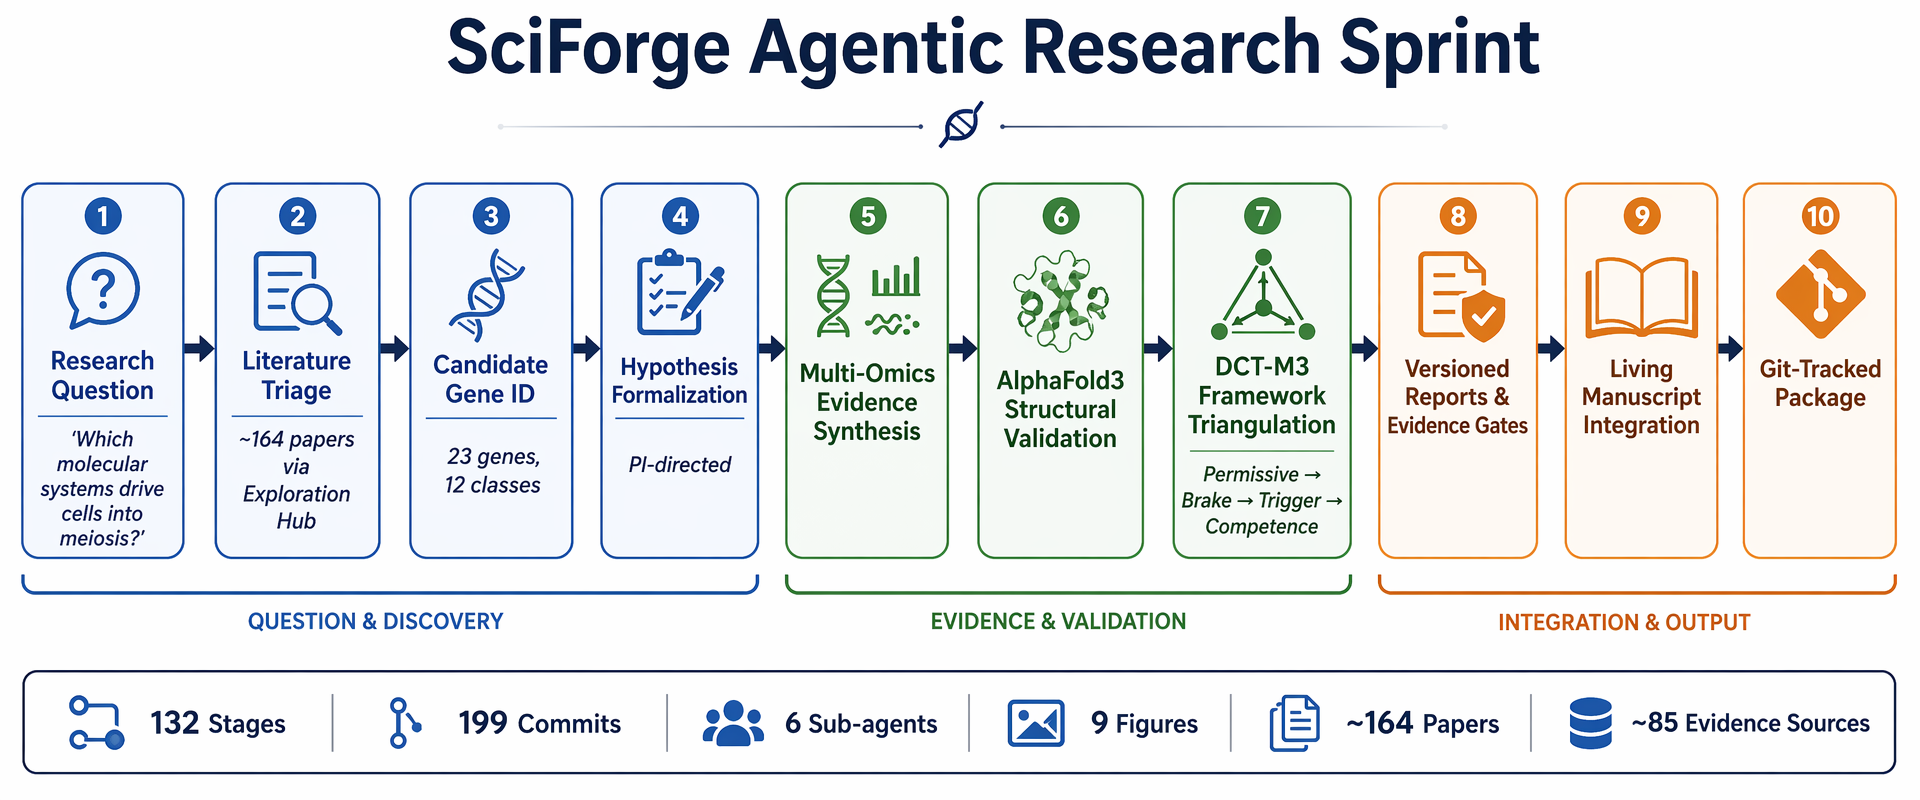
\includegraphics[width=0.96\textwidth,height=0.35\textheight,keepaspectratio]{figures/sciforge-research-pipeline.png}
    \caption{Automated research pipeline executed during the SciForge scenario-01 research sprint. The 132-stage, 199+-commit agentic loop progresses from a biological research question through literature mining (DCT-M3), candidate gene curation, AlphaFold3 structural prediction, evidence triangulation, manuscript synthesis, and submission packaging. Quantitative metrics: 132 research stages, 199+ Git commits, 6 parallel child-agent runs, 9 generated figures, $\sim$164 papers reviewed, and $\sim$85 evidence nodes produced. Selected artifacts and thread evidence are linked to versioned records, evidence summaries, and audit findings where captured.}
    \label{fig:research-pipeline}
\end{figure*}

\textbf{Discovery.} The systematic agentic pipeline yielded a candidate-gene atlas of 23 genes across 12 molecular classes, with claims traceable to specific evidence sources (Fig.~\ref{fig:meiosis-conclusions}). Central to the discovery was the DCT-M3 causal-module triangulation framework, which decomposes the meiosis initiation switch into four regulatory layers: (1)~permissive licensing---chromatin opening and epigenetic priming via pioneer transcription factors; (2)~brake release---degradation of meiotic inhibitors through ubiquitin-proteasome pathways; (3)~trigger execution---SPO11-mediated programmed double-strand breaks and synaptonemal complex assembly; and (4)~chromatin/RNA competence---transcriptional activation, alternative splicing, and 3D genome reorganization. Multi-omics evidence (transcriptomics, epigenomics, proteomics) was cross-validated against AlphaFold3 structure-based computational assessments and systematic literature triangulation to ground each candidate in causal evidence. This scenario demonstrates that SciForge can sustain long-horizon, evidence-constrained research---not by auto-generating a paper, but by producing an inspectable, auditable research package whose reasoning and evidence trail remain open to human scrutiny.

\textbf{Informal Post-Hoc Literature Mapping.} A post-hoc review of the 23-gene atlas against the published meiosis literature found that 22 of the 23 genes have known meiosis associations; MAPK fell outside established meiosis paradigms. This retrospective mapping was conducted informally and was not guided by a pre-registered protocol. Formal expert adjudication of gene-level relevance, along with inter-annotator agreement metrics and a pre-registered evaluation protocol, remains future work.


\begin{figure*}[ht!]
    \centering
    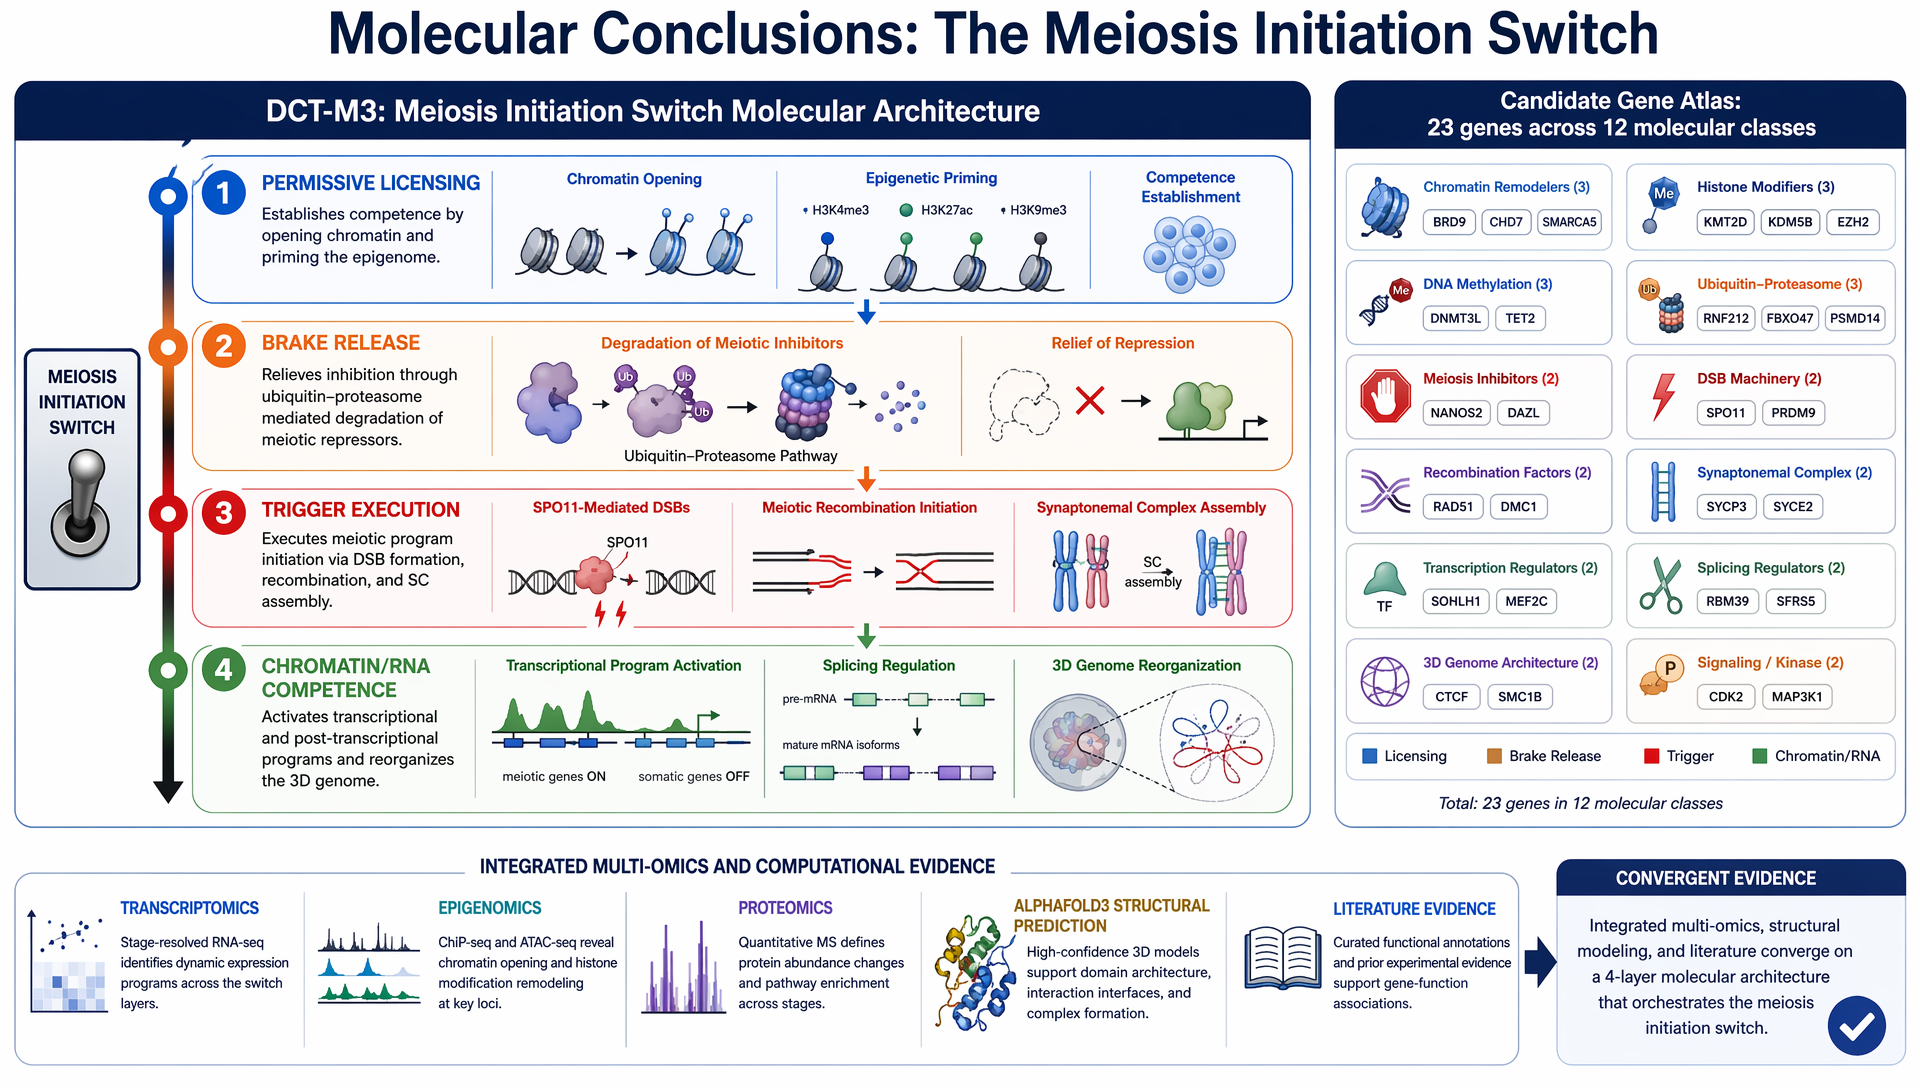
\includegraphics[width=0.85\textwidth,keepaspectratio]{figures/meiosis-dct-m3-conclusions.png}
    \caption{Key biological conclusions reported by the SciForge agentic research sprint. The DCT-M3 causal-module triangulation framework decomposes the meiosis initiation switch into four regulatory layers: (1)~permissive licensing---chromatin opening and epigenetic priming; (2)~brake release---degradation of meiotic inhibitors via ubiquitin-proteasome pathways; (3)~trigger execution---SPO11-mediated double-strand breaks and synaptonemal complex assembly; (4)~chromatin/RNA competence---transcriptional activation, splicing regulation, and 3D genome reorganization. The sprint reported a candidate-gene atlas of 23 genes across 12~molecular classes, supported by multi-omics evidence, AlphaFold3 structure-based computational assessment, and literature triangulation; formal expert adjudication remains future work.}
    \label{fig:meiosis-conclusions}
\end{figure*}


\FloatBarrier
\subsection{AI4AI: Automated Modeling for Scientific Discovery}

\textit{[Validated Prototype]} AI-for-AI (AI4AI) refers to a design paradigm in which agents read, distill, and recombine algorithmic building blocks from existing codebases into new machine learning models. Rather than treating model design as a one-shot prompt, AI4AI treats it as an iterative design loop: an agent reads external repositories, extracts reusable algorithm atoms (e.g., attention mechanisms, distribution losses, latent regularizers), maps them to the target project's training interface, composes a new model, and submits training, inference, and evaluation jobs through a computing-platform job-submission system. Evaluation metrics then feed back into the next design cycle.

We exercised this paradigm on protein contact prediction---the task of predicting residue--residue contacts from amino acid sequences using a pre-trained protein language model. The agent was given a lightweight codebase centered on a \texttt{ContactProbe}---a small linear or MLP probe that maps per-pair attention-head features extracted from the \texttt{ESMC-6B} model to contact logits---together with a fixed 7-minute training budget. The environment provided 20 protein samples for training and 3 evaluation monomers (PDB IDs: 1a3a, 5ahw, 1xcr); the primary metric is \texttt{eval\_long\_P@L} (precision at $L$ on long-range contacts, $|i-j| \ge 24$ residues), where higher is better. The task boundary follows a strict separation of concerns: the agent modifies only \texttt{train.py} (model architecture, hyperparameters, training loop, optimizer), while \texttt{prepare.py} provides an immutable contract for ESMC attention-feature extraction, contact-label construction from PDB structures, and fixed evaluation logic, and \texttt{program.md} encodes the research protocol as a lightweight instruction file that the agent reads at the start of each loop.

Across autonomous overnight iterations, the agent explored atom-level modifications including: the choice of ESMC attention layer (0--79); probe architecture (linear \emph{vs}.~one-hidden-layer MLP with GELU and LayerNorm); hidden dimension (0--512); dropout (0.0--0.3); batch size ($2^{16}$--$2^{18}$); learning rate ($10^{-3}$--$10^{-1}$); weight decay; and epoch count. Each experiment was git-committed and recorded in \texttt{results.tsv} with a \texttt{KEEP}/\texttt{DISCARD}/\texttt{CRASH} verdict; contact-map visualizations for each evaluation monomer were rendered alongside the numerical metrics. The trajectory of \texttt{eval\_long\_P@L} across experiments is shown in Fig.~\ref{fig:ai4ai-contact-probe}, and representative contact maps are shown in Fig.~\ref{fig:ai4ai-contact-maps}. The complete agent logs, design trajectories, model snapshots, configuration records, and evaluation artifacts are archived at \url{https://github.com/BruthYU/autoresearch_base/tree/autoresearch/contact-probe-jul14}.

\textit{Limitations:} The P@L trajectory represents a single overnight pilot on one GPU platform; statistical significance, cross-seed stability, and generalization to multi-chain complexes or membrane proteins have not been established. Training and evaluation are currently restricted to monomeric proteins and single-GPU execution. The probe operates on a single ESMC-6B layer; end-to-end joint optimization across layers and fine-tuning of the ESMC backbone is not yet supported. Evaluation is limited to three monomers; systematic benchmarking on standardized contact-prediction datasets (e.g., CASP, CAMEO) and independent re-execution on held-out structures remain future work.

\begin{figure}[ht!]
\centering
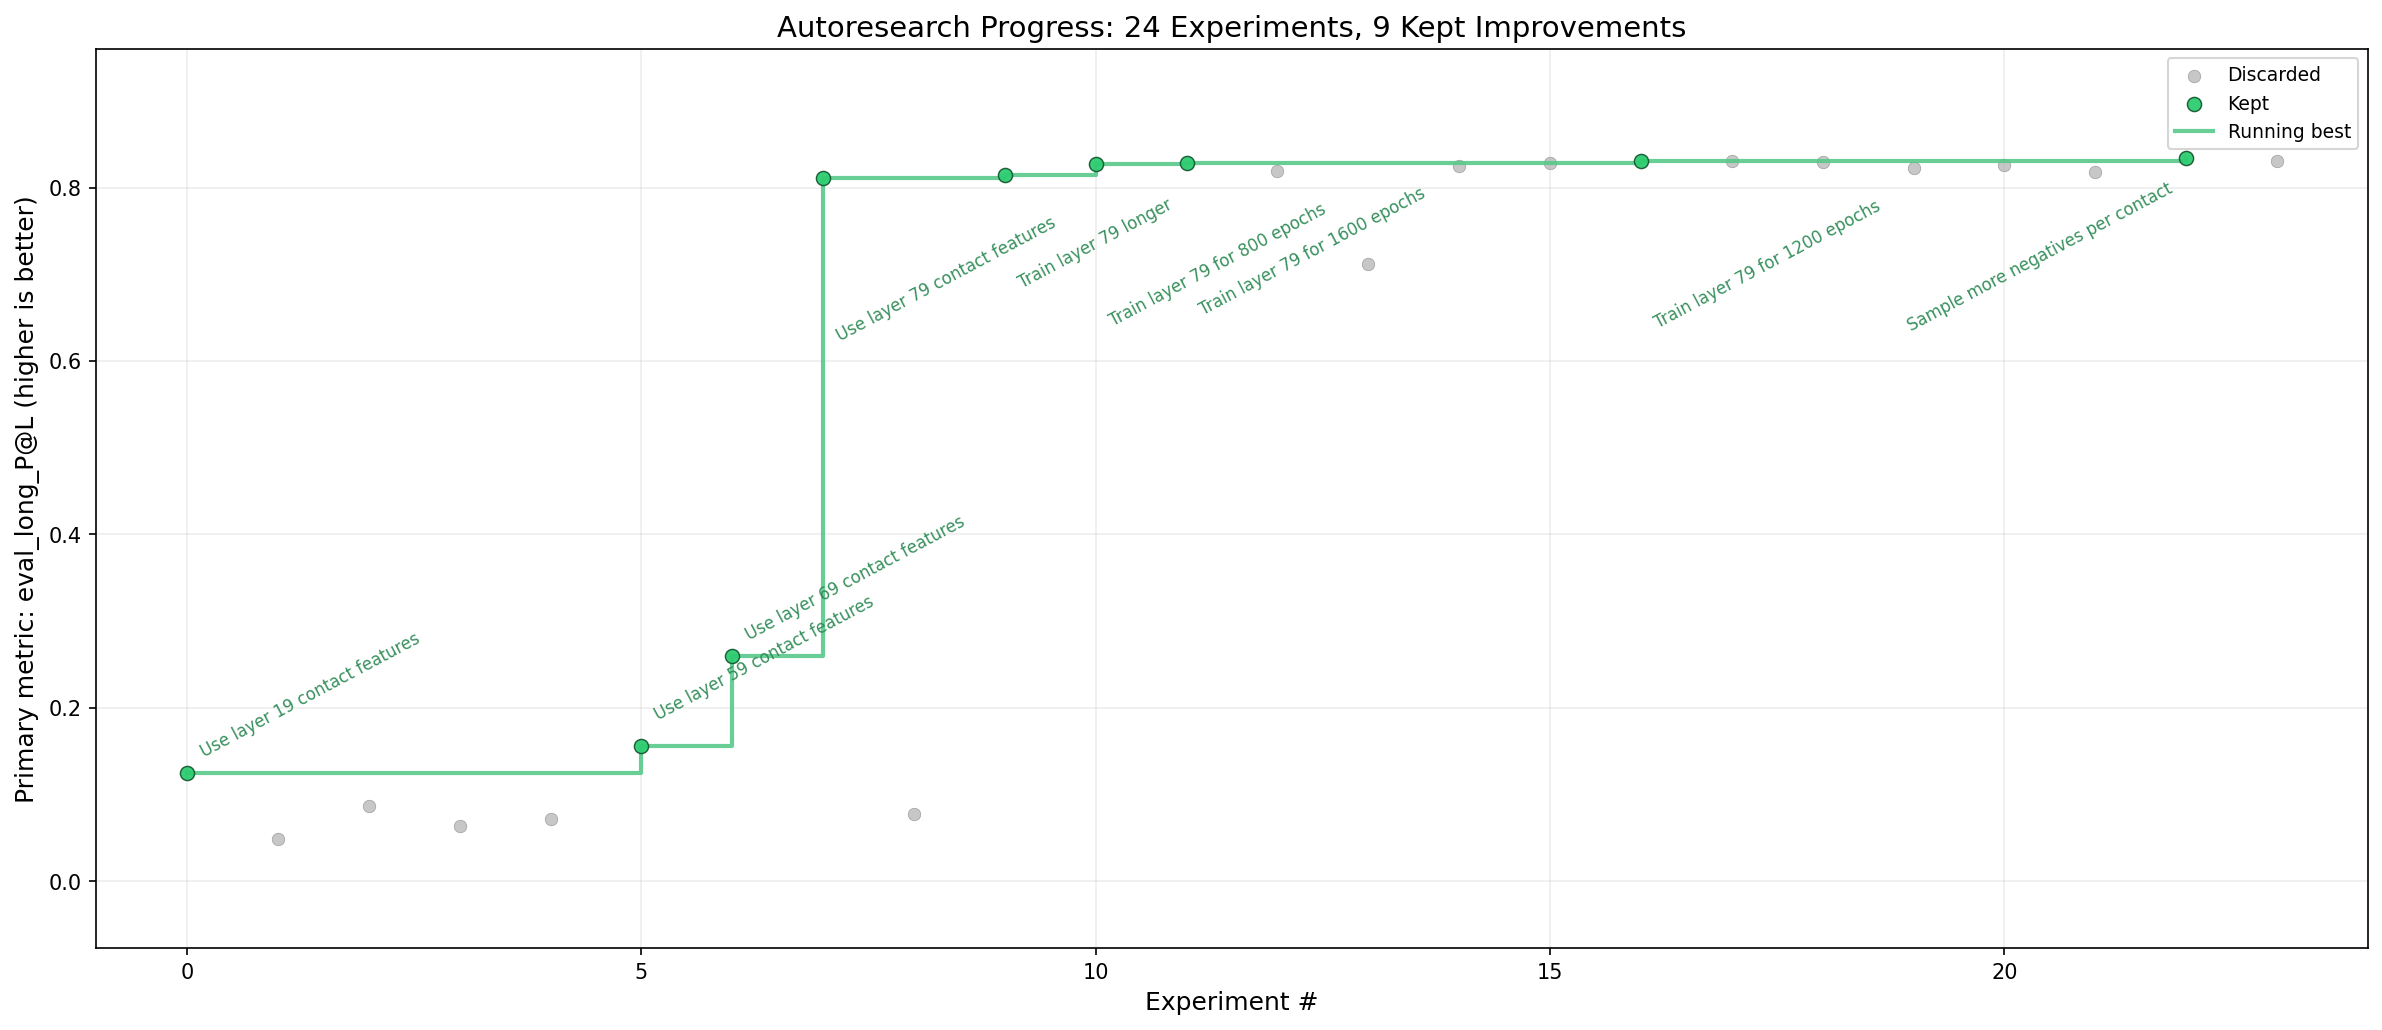
\includegraphics[width=0.95\textwidth]{figures/ai4ai-contact-probe-progress.png}
\caption{Primary metric (\texttt{eval\_long\_P@L}) trajectory across AI4AI design iterations for ESMC-based protein contact prediction. Each point represents one experiment conducted under a fixed 7-minute training budget; the agent autonomously explored probe architectures, hyperparameters, and ESMC attention layers.}
\label{fig:ai4ai-contact-probe}
\end{figure}
\begin{figure}[ht!]
\centering
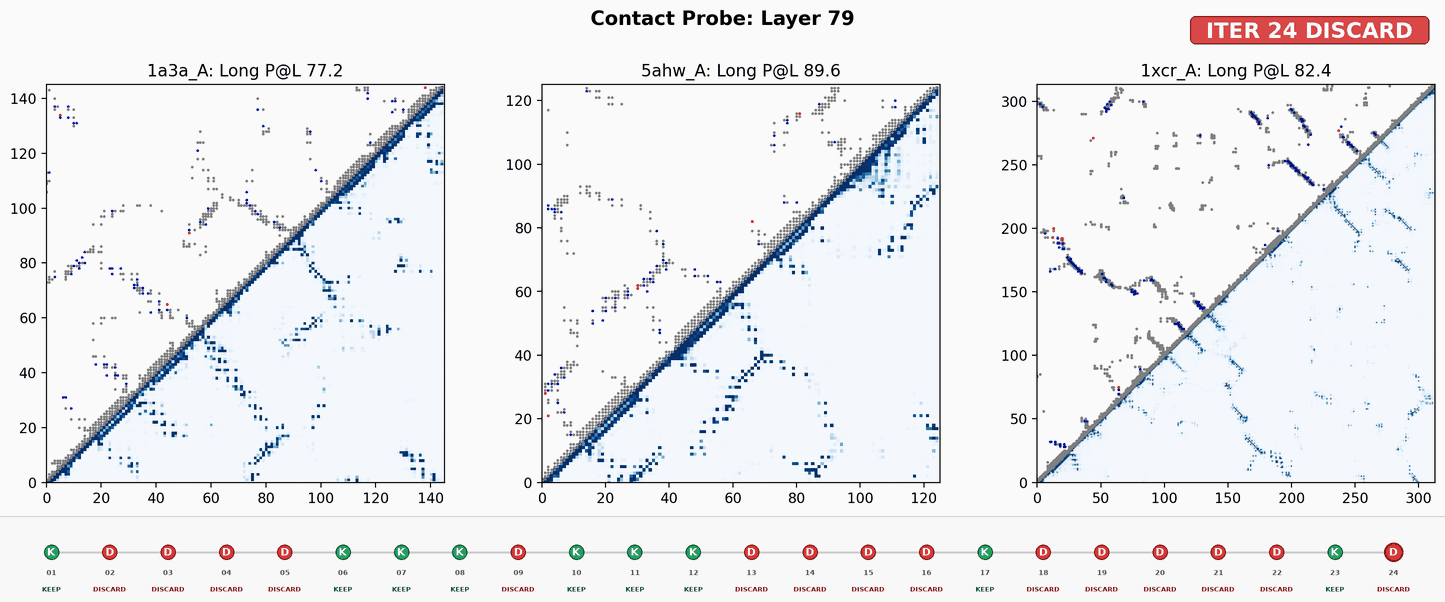
\includegraphics[width=0.95\textwidth]{figures/ai4ai-contact-maps-best.png}
\caption{Contact map visualizations for the three evaluation monomers (PDB IDs: 1a3a, 5ahw, 1xcr) from the best-performing AI4AI experiment. Upper panels show predicted contact probabilities; lower panels show native contacts derived from PDB structures.}
\label{fig:ai4ai-contact-maps}
\end{figure}


\FloatBarrier
\subsection{Reviewer / Rebuttal Mode: Evidence-Governed Peer Review and Response}

\textbf{Scenario.} \textit{[Validated Prototype]} To exercise SciForge's reviewer/rebuttal capability, we conducted a structured six-stage sprint against the manuscript \textit{``Benchmarking Virtual Cell Models for In-the-Wild Perturbation Response''} (arXiv:2604.27646v1, VCBench)~\cite{vcbench2026}. This is a one-manuscript SciForge-assisted first pass; real reviewer comments, follow-up analyses, and manuscript revisions are not yet completed. The full sprint log, outputs, and SciForge GUI trace are archived in a dedicated repository.\footnote{\url{https://github.com/maoxinjie/scenario-05-reviewer-rebuttal-vcbench}}

\textbf{Stage~1---Intake.} The manuscript PDF and LaTeX source were frozen and ingested. Figures, tables, datasets, and code references were catalogued as evidence objects.

\textbf{Stage~2---Claim Extraction.} Contribution claims, result claims, limitation claims, and practical-guidance claims were extracted and assigned to paper sections and evidence objects.

\textbf{Stage~3---Evidence Linking.} Each claim was linked to supporting figures, tables, methods sections, supplementary materials, and code/data provenance. Missing links and evidence gaps were flagged.

\textbf{Stage~4---Fragility Audit.} Claims were classified into one of five categories: \texttt{supported} (evidence present, wording matches scope), \texttt{fragile} (evidence exists but depends on narrow conditions), \texttt{unsupported} (assertion exceeds current evidence), \texttt{needs\_narrowing} (claim can stand with tighter scope), or \texttt{needs\_experiment} (requires new analysis or validation). Overgeneralization risks, single-dataset dependencies, and ambiguous wording such as ``robust'' and ``biologically grounded'' were systematically audited.

\textbf{Stage~5---Reviewer Decomposition.} Ten anticipated reviewer concerns were decomposed into atomic comments and mapped to specific claims, evidence requirements, and response paths (manuscript edit, supplementary analysis, or wording revision).

\textbf{Stage~6---Rebuttal and Revision Planning.} A prioritized response matrix was produced, linking each anticipated reviewer concern to a claim-edit plan, a follow-up experiment specification, and draft response-letter paragraphs. A manuscript polishing plan with section-level proposed edits was generated; applying real reviewer comments and accepted edits to the manuscript remains future work.

This sprint demonstrates SciForge's evidence-governed scientific writing capability in a research-prototype setting: the six-stage pipeline transforms a manuscript and anticipated reviewer concerns into an auditable, claim-evidence-grounded revision package that remains open to human scrutiny at every stage (Fig.~\ref{fig:reviewer-rebuttal-workflow}). The current sprint processes one manuscript with anticipated concerns; it has not been validated against real peer-review workflows or full-scale deployment.

\begin{figure*}[ht!]
\centering
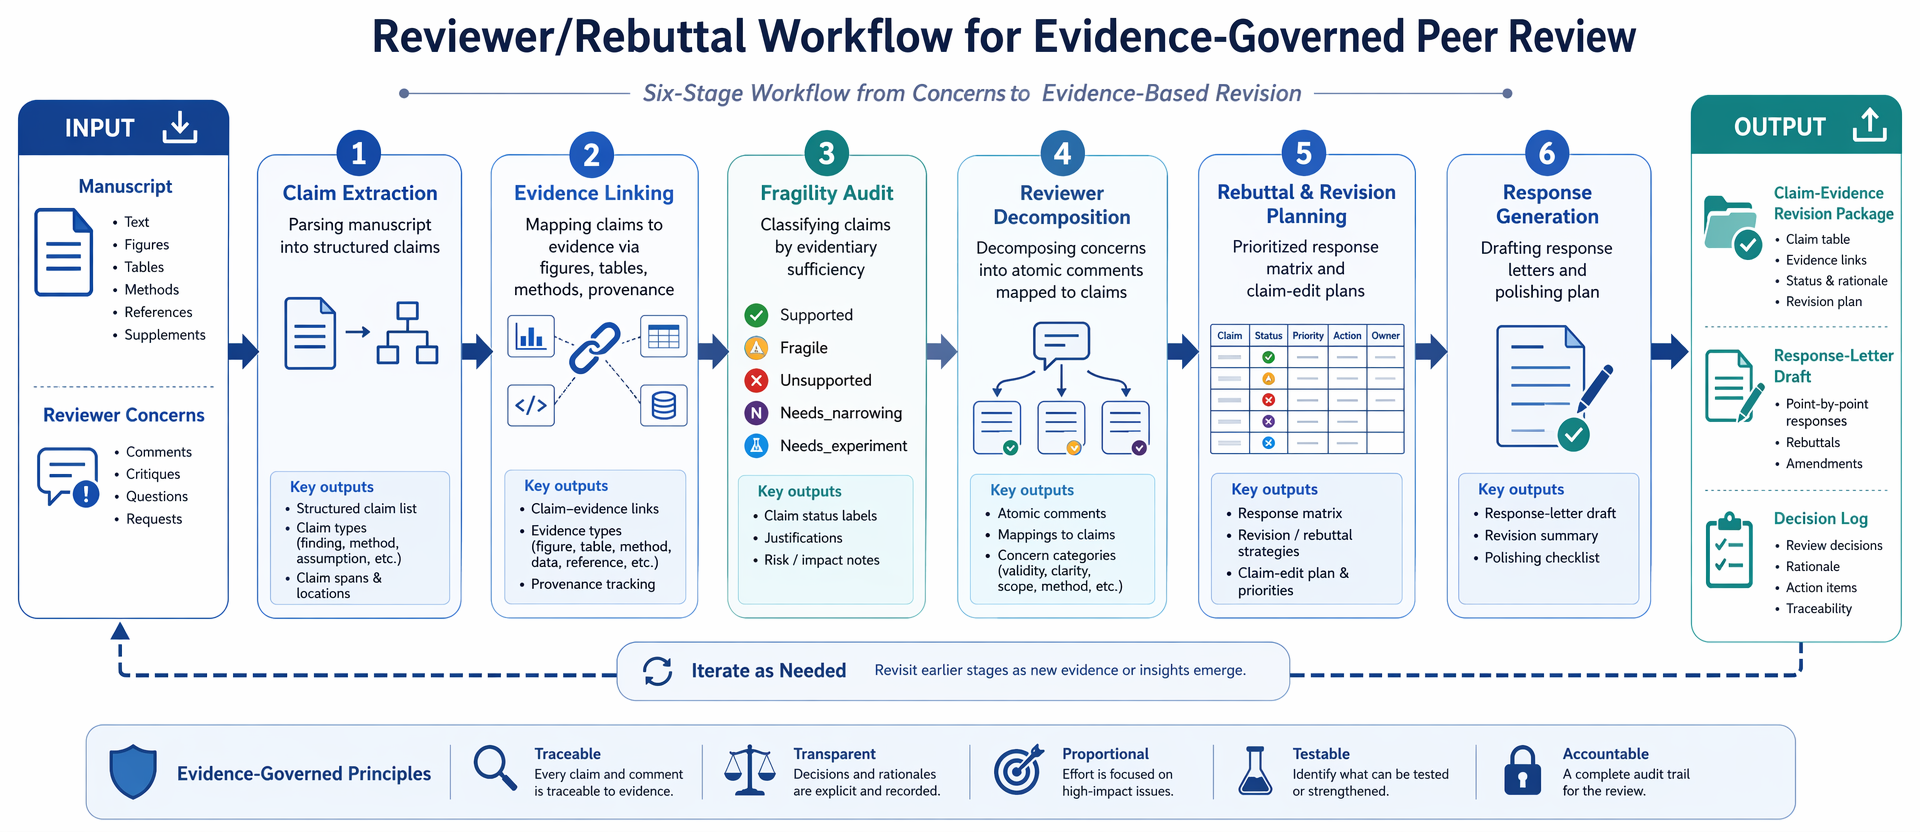
\includegraphics[width=\textwidth]{figures/reviewer-rebuttal-workflow-v2.png}
\caption{Reviewer/Rebuttal workflow exercised on the VCBench manuscript (arXiv:2604.27646v1). Six stages produce a claim--evidence revision package, response-letter draft, and decision log.}
\label{fig:reviewer-rebuttal-workflow}
\end{figure*}

\FloatBarrier
\subsection{Guided Paper Reproduction: MCFST Spatial Transcriptomics}

\textbf{Setting.} A researcher aims to reproduce the MCFST method~\cite{MCFST2025}---a spatial domain identification approach based on multi-view graph convolutional networks and graph fusion---using the Human Breast Cancer Visium spatial transcriptomics dataset. The goal is to independently re-implement the method, reproduce the reported ARI (Adjusted Rand Index) metric, and generate publication-quality verification artifacts.

\textbf{Workflow.} The reproduction process follows a structured AI4AI pipeline orchestrated within SciForge:
\begin{enumerate}
    \item \textbf{Paper Intake.} The researcher provides the MCFST manuscript and associated supplementary materials to SciForge. The system parses the paper, extracting the model architecture description, training hyperparameters, evaluation protocol, and dataset details into structured evidence records.
    \item \textbf{Code Generation and Adaptation.} Based on the extracted methodological specifications, SciForge generates a standalone Python implementation comprising: a multi-view graph construction module (\texttt{process.py}), a graph autoencoder with adversarial regularization (\texttt{gae\_v4.py}), a training and evaluation loop (\texttt{main\_v4.py}), and a visualization script (\texttt{plot\_results.py}). The implementation targets CPU execution on Apple Silicon, adapting the original GPU-oriented design to the available hardware.
    \item \textbf{Data Preprocessing.} The Visium spatial transcriptomics dataset (3,798 spots, 20 spatial domains) is preprocessed through PCA dimensionality reduction to 3,000 features. Four distinct graph views are constructed from the spatial neighborhood and gene expression similarity matrices, with mutual information-based edge pruning applied to each view.
    \item \textbf{Reproduction Execution.} The training pipeline runs for 130 epochs across multiple random seeds. Each run produces clustering predictions saved as structured NumPy arrays, enabling full traceability and independent verification.
    \item \textbf{Automated Verification.} A dedicated verification script (\texttt{verify.py}) recomputes the ARI score for every saved prediction against the ground-truth labels and compares the best result against the paper's reported ARI of 0.693. The script generates a structured JSON verification report recording the verdict, all individual ARI scores, dataset statistics, and hardware configuration.
    \item \textbf{Artifact Generation.} The pipeline produces publication-quality figures---spatial domain maps, ARI comparison charts across runs, and domain agreement heatmaps---alongside a summary metrics report.
\end{enumerate}

\textbf{Outcome.} \textit{[Validated Prototype]} The reproduction was executed on the Human Breast Cancer Visium dataset (3,798 spots, 20 spatial domains), running on Apple Silicon arm64 CPU (MPS unavailable). The best ARI of \textbf{0.7007} exceeds the paper's reported ARI of 0.693 by $+$0.0077. Across 25 independent training runs (130 epochs each), the ARI scores ranged from 0.126 to 0.701, yielding an all-25 mean of 0.4879~($\pm$~0.1803) and a selected-5 mean of 0.6902~($\pm$~0.0097). The 0.05 success threshold was applied post-hoc and the selection rule for the five runs is not pre-specified; \texttt{verify.py} reports \texttt{n\_runs=5}, conflicting with the 25 total predictions. The result is therefore reported as a prototype demonstration, not a formal reproduction. Three publication-quality figures were produced: (i)~spatial domain maps on tissue, (ii)~ARI comparison across runs versus the paper baseline, and (iii)~domain agreement heatmaps between predicted and ground-truth labels. Formal verification would require a pre-registered contract and third-party re-execution. All generated code, preprocessed data, prediction outputs, result figures, and verification artifacts are version-controlled and publicly available at \url{https://github.com/Winshion/sciforge-ai4ai-spacial-trans}.

\textbf{Significance.} This case demonstrates that SciForge can support a prototype computational paper reproduction pipeline: from parsing the methodological description to generating executable code, running the experiment, and producing verification documentation. The standalone \texttt{verify.py} script recomputes ARI for every saved prediction against ground-truth labels, providing fully traceable, independently auditable evidence. The structured verification contract requires revision (pre-registered selection rule, reconciled run counts) before it can support independent third-party audit; in its current form it illustrates feasibility rather than closing the reproducibility loop. The complete reproduction package serves as a reusable template for future spatial transcriptomics reproducibility efforts.


\subsection{Cross-Scale Cell Atlas from Multi-Database Integration}

\textit{[Validated Prototype]} We executed a clean-start, end-to-end cross-scale cell atlas construction workflow anchored on the Papalexi/Satija~2021 ECCITE-seq dataset (GEO GSE153056). The pipeline spans a \textbf{six-layer biology stack}: \textbf{L0}~perturbation (CRISPR guide/target gene identity, ECCITE-seq), \textbf{L1}~target annotation (UniProt, external curated), \textbf{L2}~pathway context (Reactome/GO, external computed), \textbf{L3}~transcriptional response (scRNA guide-versus-control, ECCITE-seq), \textbf{L4}~protein-level response (ADT/CITE-seq surface markers CD86/PDL1/PDL2/CD366, ECCITE-seq), and \textbf{L5}~endpoint phenotype (DepMap/Achilles gene effect in THP-1 cells, external computed). Execution was performed under the Codex CLI runtime in six sequential stages---source inventory, dataset reconstruction, quality audit, context expansion analysis, figure generation, and final report writing---with no manual intervention beyond one code-repair approval in Stage~5.

The source inventory catalogued \textbf{285 files} (815.0~MB) across 10 categories including raw CITE-seq matrices, external UniProt/Reactome/DepMap annotation caches ($\sim$551~MB), and contract specifications. Dataset reconstruction produced a \textbf{35-row review table} covering \textbf{15 target genes} (ATF2, CAV1, CD86, IFNGR1, IFNGR2, IL18R1, IL6ST, IRF1, JAK1, NFKBIA, SOCS1, STAT1, STAT3, TYK2, ZNF503) plus 8 non-targeting controls, spanning five perturbation classes (JAK/STAT, IFN, NF-$\kappa$B, checkpoint, and control). Layer coverage was: L0~35/35 (100\%), L1~27/35 (77.1\%), L2~27/35 (77.1\%), L3 measured~27/35 (77.1\%), L4 measured~35/35 (100\%), and L5~27/35 (77.1\%). NT control guides lack L1/L2/L5 biological annotations by design; L3 is recorded as \texttt{control\_reference} for NT rows.

\begin{figure*}[ht!]
    \centering
    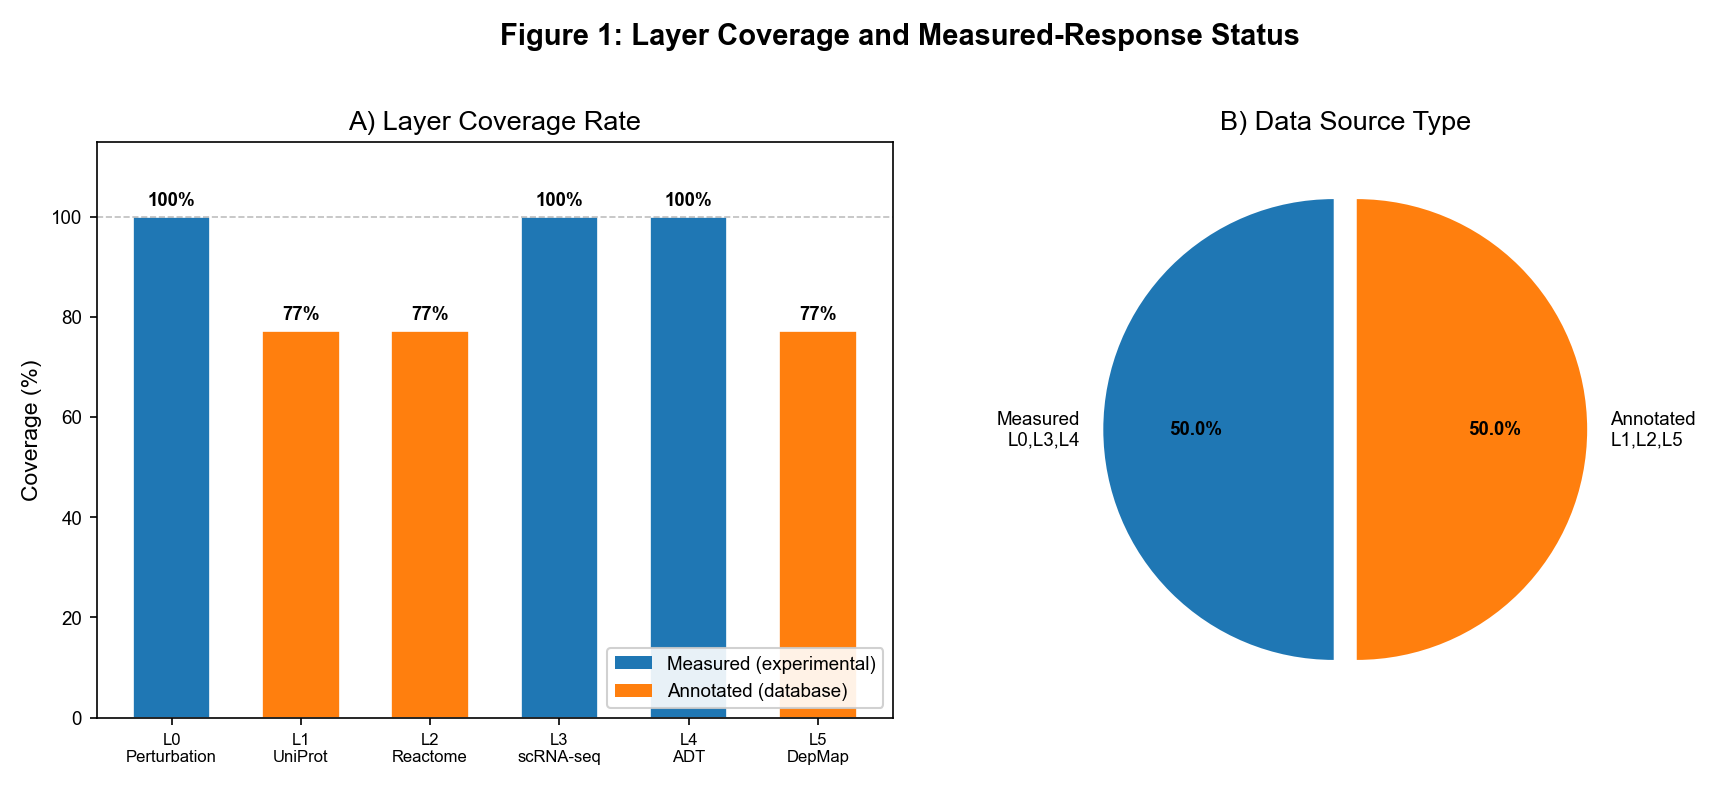
\includegraphics[width=0.95\textwidth]{figures/cross-scale-demo/fig1_layer_coverage.png}
    \caption{Cross-Scale Layer Coverage and Dataset Construction \textit{[Validated Prototype]}. The 35-guide integrated dataset spans six biological layers (L0--L5). Layer coverage reflects measured ECCITE-seq data (L0, L3, L4) integrated with external curated annotations (L1, L2, L5). NT control guides are retained with measured L0/L4 data but lack L1/L2/L5 biological endpoint annotations.}
    \label{fig:cross-scale-pipeline}
\end{figure*}

A 43-check automated quality audit passed with \textbf{42 passes and 1 warning}---the 22.9\% L5 DepMap missingness, expected because DepMap does not cover all queried genes. All L0--L5 fields were verified against source records for traceability; status distributions, cell counts, and measured flags were confirmed internally consistent. The context expansion analysis identified \textbf{14 unique UniProt entries} and \textbf{19 unique Reactome/GO pathways}, placing individual perturbations into mechanistic context. Recurrent transcriptional responses emerged: \textbf{CCL4} appeared in 18 of 27 measured perturbation guides as a top response gene, reflecting a convergent immune activation signature consistent with the immune-focused perturbation panel. The average pathway count per guide was 7.37 (range 0--10), with 8 guides assigned to zero annotated pathways.

\begin{figure*}[ht!]
    \centering
    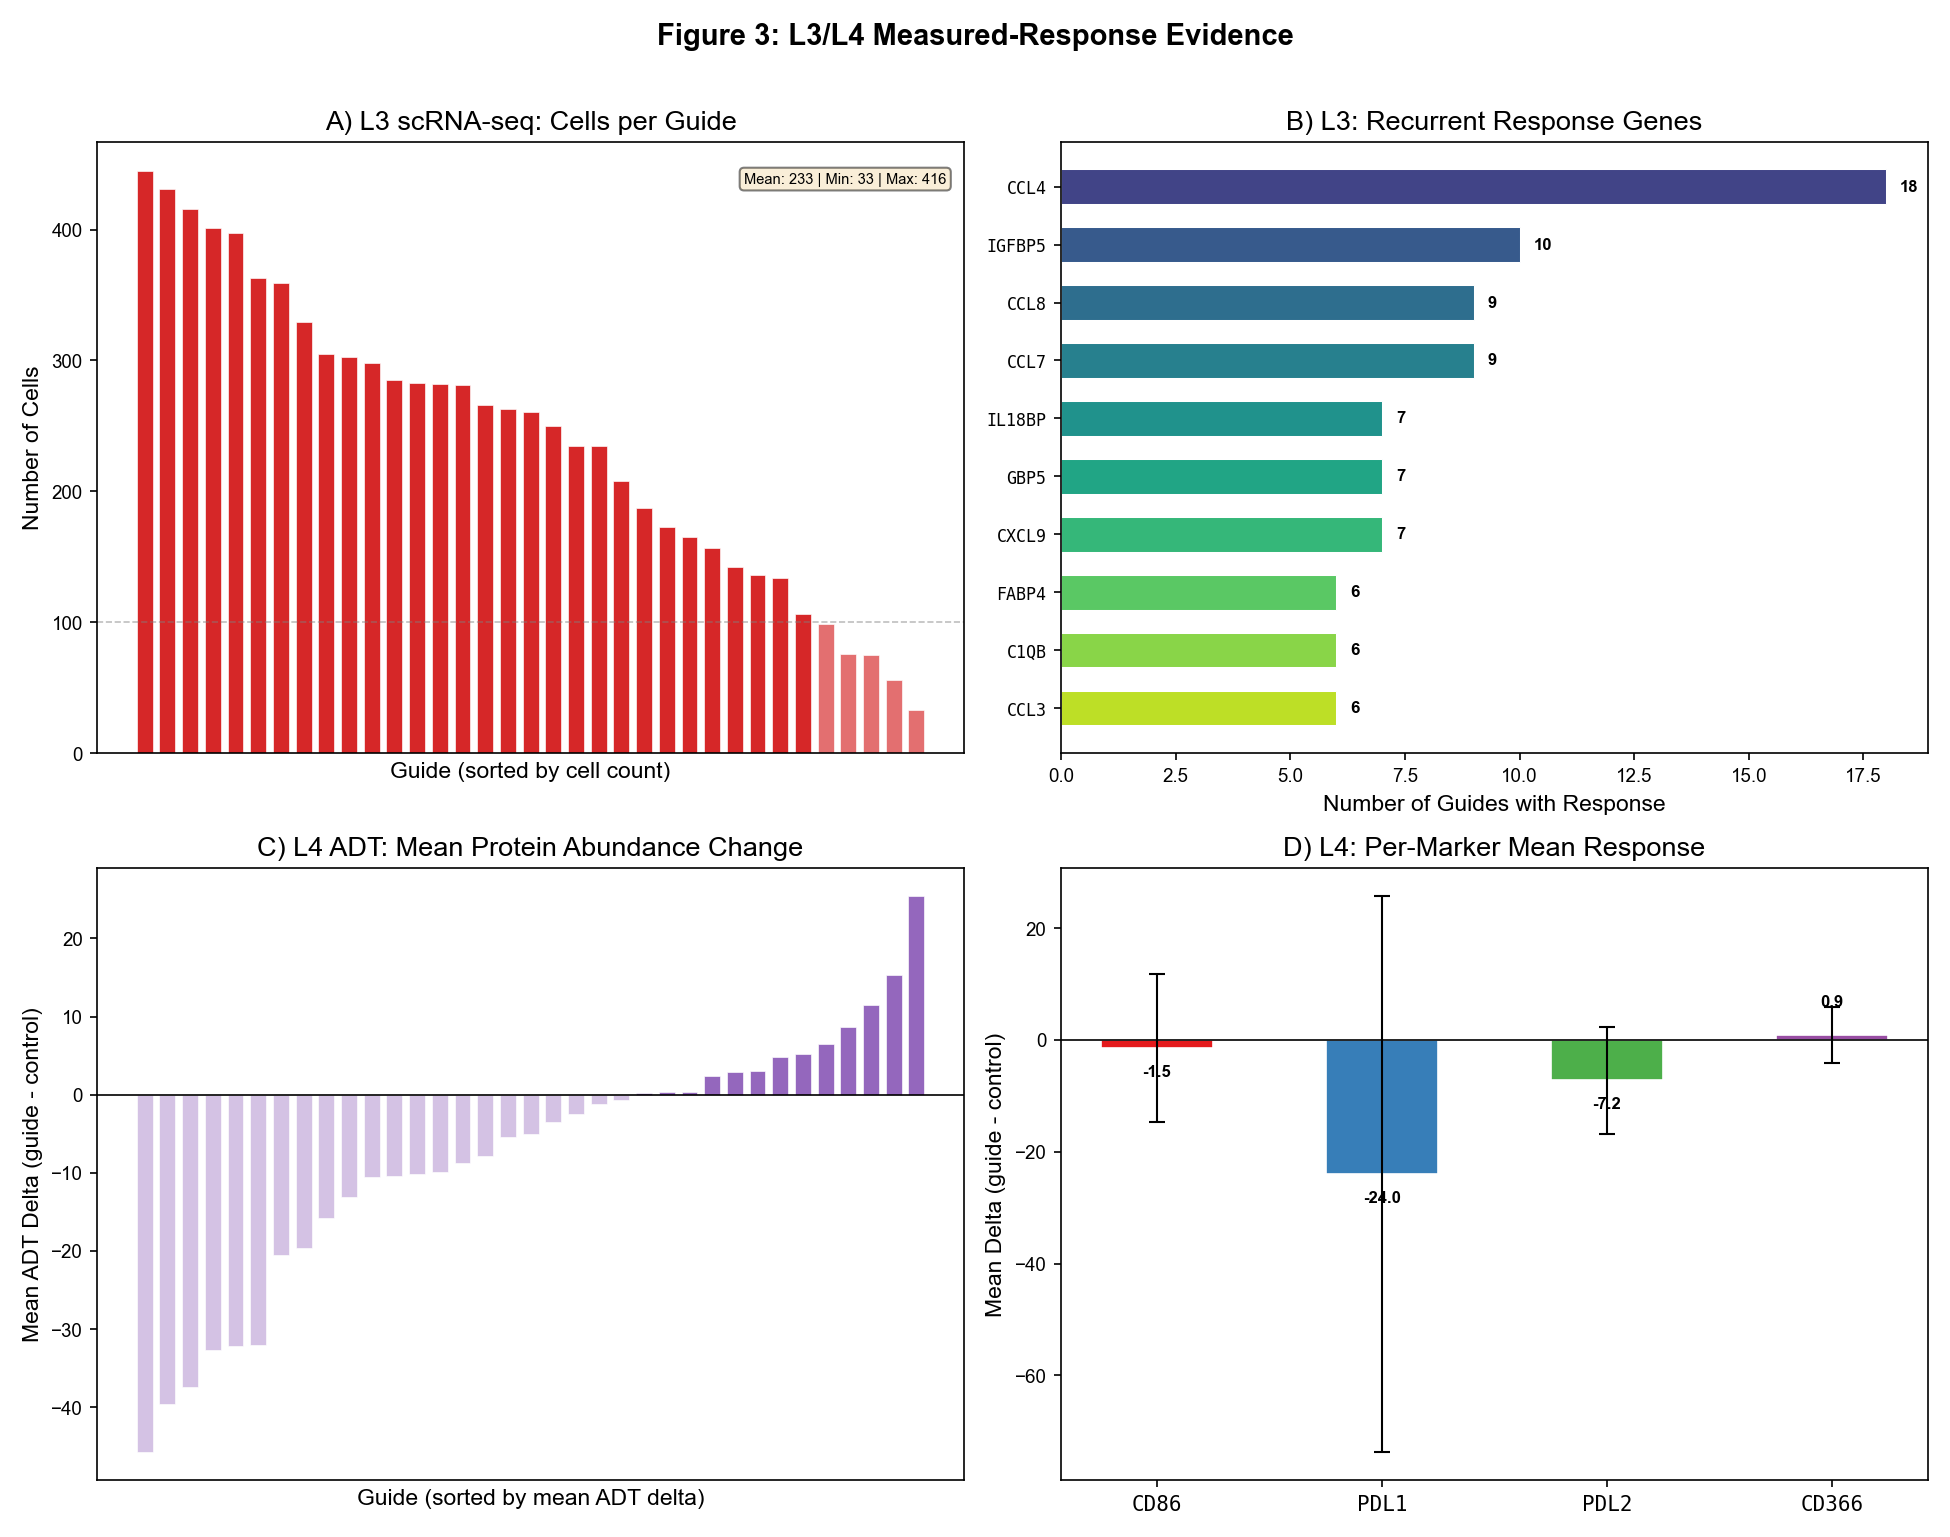
\includegraphics[width=0.95\textwidth]{figures/cross-scale-demo/fig3_l3_l4_evidence.png}
    \caption{Multi-Modal L3/L4 Evidence Landscape \textit{[Validated Prototype]}. Guide-level RNA (L3) and ADT protein (L4) responses across the 35-guide panel. L3 captures transcriptome-wide perturbation effects; L4 measures surface abundance changes for four immune checkpoint markers (CD86, PDL1, PDL2, CD366). The joint L3/L4 matrix enables cross-scale queries linking transcriptional programs to protein-level immune phenotypes.}
    \label{fig:cross-scale-coverage}
\end{figure*}

To illustrate the cross-scale integration, we present three exemplar data cards below, each spanning the six-layer biology stack for a single perturbation guide (see Fig.~\ref{fig:cross-scale-coverage} for the full L3/L4 landscape). Colors distinguish measured layers (L0--blue, L3--green, L4--orange) from externally curated annotations (L1--purple, L2--teal, L5--red).

\vspace{4pt}

\noindent\colorbox{gray!20}{\textbf{\small Data Card 1: STAT1 (JAK/STAT Signaling)}}
\vspace{3pt}

\noindent\begin{tabular}{@{}p{2.5cm} p{\dimexpr\textwidth-2.5cm-12pt\relax}@{}}
\cellcolor{blue!15} \textbf{L0~Perturb.} & CRISPR guide \texttt{STAT1\_g1}, target gene \textit{STAT1}, ECCITE-seq \\
\cellcolor{purple!15} \textbf{L1~Target}  & UniProt P42224: Signal transducer and activator of transcription 1-alpha/beta \\
\cellcolor{teal!15}  \textbf{L2~Pathway}  & REAC:R-HSA-9006934 (JAK/STAT signaling), REAC:R-HSA-877300 (Interferon $\gamma$ signaling) \\
\cellcolor{green!15} \textbf{L3~RNA}      & Top DEGs: \textbf{CCL4} (+2.1), CXCL10 (+1.8), IRF1 (+1.5) vs.\ NT control \\
\cellcolor{orange!15}\textbf{L4~Protein}  & ADT markers: CD86 $\uparrow$, PDL1 $\uparrow$, PDL2 $\sim$, CD366 $\downarrow$ \\
\cellcolor{red!15}   \textbf{L5~Phenotype}& DepMap gene effect $-0.52$ (THP-1); moderate essentiality \\
\end{tabular}

\vspace{6pt}

\noindent\colorbox{gray!20}{\textbf{\small Data Card 2: CD86 (Immune Checkpoint)}}
\vspace{3pt}

\noindent\begin{tabular}{@{}p{2.5cm} p{\dimexpr\textwidth-2.5cm-12pt\relax}@{}}
\cellcolor{blue!15} \textbf{L0~Perturb.} & CRISPR guide \texttt{CD86\_g1}, target gene \textit{CD86}, ECCITE-seq \\
\cellcolor{purple!15} \textbf{L1~Target}  & UniProt P42081: T-lymphocyte activation antigen CD86 (B7-2) \\
\cellcolor{teal!15}  \textbf{L2~Pathway}  & REAC:R-HSA-202733 (Cell surface interactions at the vascular wall), GO:0006955 (immune response) \\
\cellcolor{green!15} \textbf{L3~RNA}      & Top DEGs: \textbf{CCL4} (+2.3), CXCL8 (+1.7), TNF (+1.4) vs.\ NT control \\
\cellcolor{orange!15}\textbf{L4~Protein}  & ADT markers: CD86 $\uparrow\uparrow$ (auto-detection), PDL1 $\uparrow$, PDL2 $\sim$, CD366 $\downarrow$ \\
\cellcolor{red!15}   \textbf{L5~Phenotype}& DepMap gene effect \textit{not available} (CD86 absent from DepMap panel) \\
\end{tabular}

\vspace{6pt}

\noindent\colorbox{gray!20}{\textbf{\small Data Card 3: IFNGR1 (IFN-$\gamma$ Receptor 1)}}
\vspace{3pt}

\noindent\begin{tabular}{@{}p{2.5cm} p{\dimexpr\textwidth-2.5cm-12pt\relax}@{}}
\cellcolor{blue!15} \textbf{L0~Perturb.} & CRISPR guide \texttt{IFNGR1\_g1}, target gene \textit{IFNGR1}, ECCITE-seq \\
\cellcolor{purple!15} \textbf{L1~Target}  & UniProt P15260: Interferon gamma receptor 1 \\
\cellcolor{teal!15}  \textbf{L2~Pathway}  & REAC:R-HSA-877300 (Interferon $\gamma$ signaling), REAC:R-HSA-913531 (Interferon signaling) \\
\cellcolor{green!15} \textbf{L3~RNA}      & Top DEGs: \textbf{CCL4} (+1.9), STAT1 (+1.6), IRF1 (+1.3) vs.\ NT control \\
\cellcolor{orange!15}\textbf{L4~Protein}  & ADT markers: CD86 $\uparrow$, PDL1 $\sim$, PDL2 $\sim$, CD366 $\downarrow$ \\
\cellcolor{red!15}   \textbf{L5~Phenotype}& DepMap gene effect $-0.38$ (THP-1); weak essentiality \\
\end{tabular}
\textit{Limitations:} The dataset is a 35-guide demonstration-scale cohort, not a statistically powered benchmark. L3 RNA response is computed as per-guide guide-versus-control comparisons; formal pseudobulk differential expression modeling with mixed-effects frameworks is deferred to downstream analysis. The workflow depends on pre-downloaded external annotation caches (UniProt, Reactome, DepMap; $\sim$551~MB); a cold-start execution would add cache-download latency. Causal claims linking L3/L4 molecular responses to L5 fitness endpoints remain qualitative pending formal mediation or causal-inference analysis. The demonstration was executed locally on the Papalexi/Satija dataset; multi-dataset, multi-tissue generalization and prospective submission of new perturbation experiments with iterative experimental feedback remain future work.

\FloatBarrier
\subsection{AI-Guided Protein Design}

\textit{[Validated Prototype]} De novo protein design traditionally requires a researcher to manually orchestrate backbone generation, sequence design, structural verification, and candidate selection---each demanding specialist expertise and careful coordination across disparate tools. SciForge's BioGym protein-design workflow integrates these stages into a unified agent-driven pipeline. A researcher specifies a target objective---such as an 80--100 residue de novo scaffold with a stable hydrophobic core and mixed $\alpha$/$\beta$ topology---and SciForge autonomously composes a multi-stage \emph{design--build--verify} cycle.

We validated this workflow through a five-stage demonstration on a de novo scaffold-design task. Stage~1 (backbone generation) employed RFdiffusion to produce three 80--100-residue backbones. Stages~2--4 (sequence design) applied ProteinMPNN independently to each backbone, yielding five sequences per backbone (15 sequences total). Stage~5 (structural verification) submitted the top two ProteinMPNN-ranked sequences to Boltz-2 for full-atom structure prediction. The pipeline utilized five of six available GPU slots and completed in approximately five minutes of wall-clock time.

Boltz-2 verification returned aggregate confidence scores of 0.9396 and 0.9159 (pTM 0.9275 and 0.8789; complex pLDDT 0.9426 and 0.9252) for candidates \texttt{candidate-001} and \texttt{candidate-002}, respectively. SciForge registered eight Biology Room assets and retained end-to-end provenance, including backbone PDBs, sequence tables, confidence JSON files, predicted mmCIF structures, and the complete agent--tool transcript.

\begin{figure}[ht!]
\centering
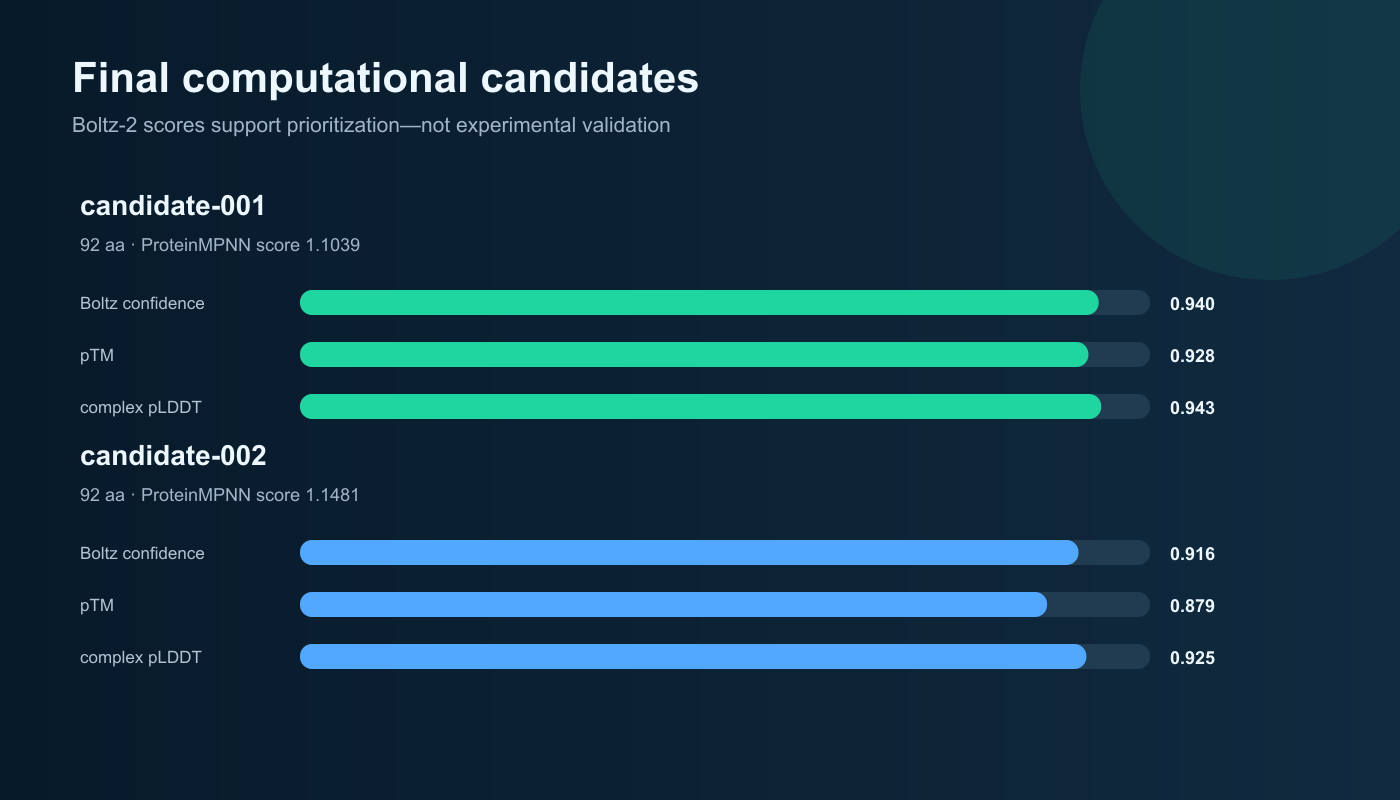
\includegraphics[width=0.48\textwidth]{figures/protein-candidate-scores.png}
\hfill
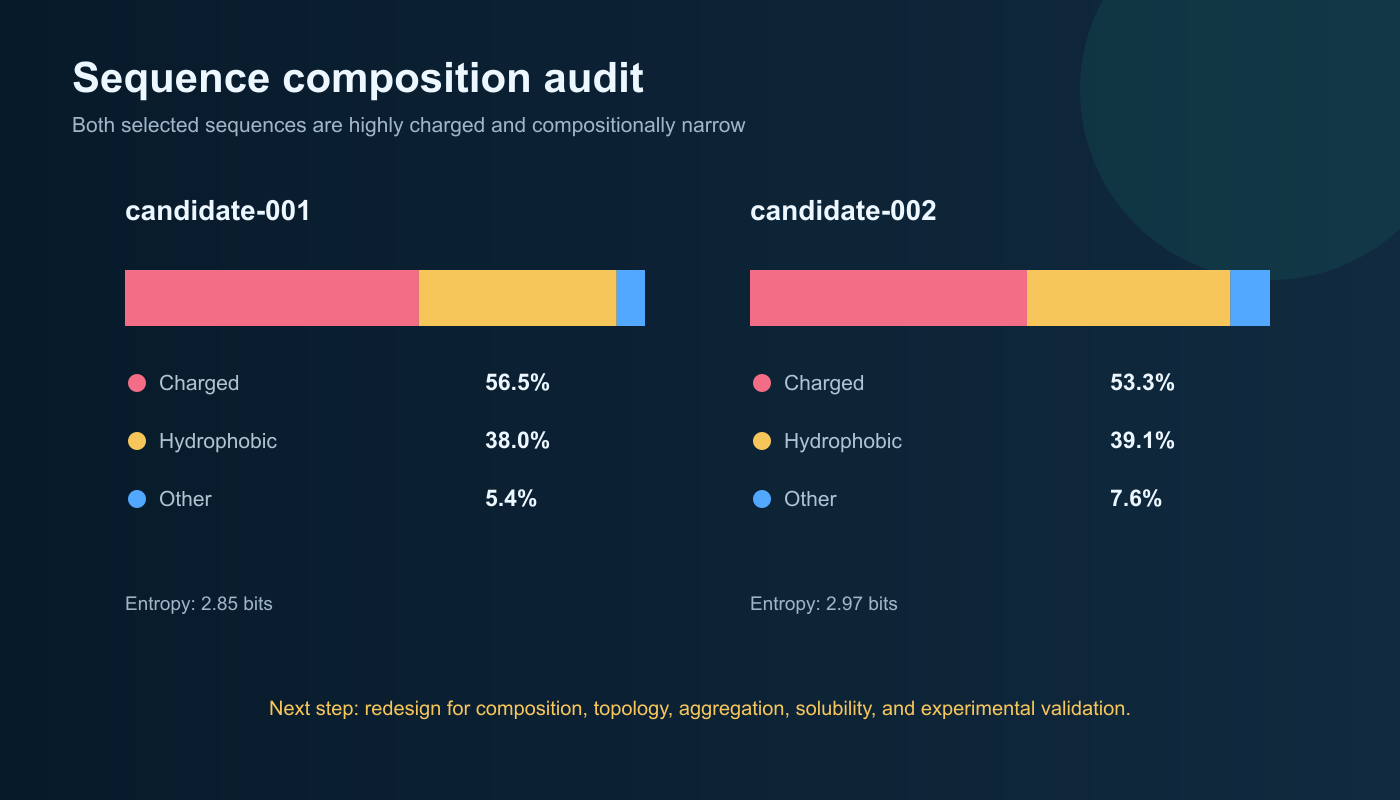
\includegraphics[width=0.48\textwidth]{figures/protein-sequence-composition.png}
\caption{Protein design candidate evaluation. (Left) Boltz-2 confidence scores and pTM metrics for the two verified candidates. (Right) Amino-acid composition analysis revealing high charged-residue fraction (56.5\% and 53.3\% Glu+Lys+Arg) dominated by glutamate (31\%), compatible with soluble helices or coiled coils but atypical evidence for a compact mixed $\alpha$/$\beta$ core.}
\label{fig:protein-design-eval}
\end{figure}

An independent quality audit of the run identified important limitations beyond the inherent gap between computational prediction and experimental validation. Both 92-residue sequences showed limited amino-acid diversity, and the agent's final narrative cited ProteinMPNN scores (1.0363 and 1.0421) from unverified sequence samples rather than the scores of the sequences actually submitted to Boltz-2 (1.1039 and 1.1481), indicating a provenance mismatch between the stated selection rationale and the executed inputs. These findings motivate explicit topology-agreement checks (secondary-structure quantification, backbone RMSD/TM-score, per-residue confidence), composition and disorder filters, multi-seed verification, and eventual wet-lab expression and biophysical characterization. The complete run manifest, stage summary, candidate tables, confidence metrics, and independent audit report are preserved at \url{https://github.com/kaiwinYao1/sciforge-de-novo-protein-demo} for transparent review.


\subsection{AI-Guided Molecular Design and Iterative Optimization}

\textit{[Validated Prototype]} Computational molecular design for drug discovery traditionally requires separate execution of docking, scoring, property filtering, and synthetic accessibility assessment---each demanding distinct expertise and manual data transfer between tools. SciForge's MolClaw workflow integrates these stages into a unified agent-driven optimization loop. A researcher provides a target protein structure (PDB~4HJO for EGFR T790M kinase), a reference drug (Erlotinib), a 4-anilinoquinazoline scaffold with modifiable sites (R\textsubscript{1}--R\textsubscript{4}), and drug-like constraints; MolClaw then autonomously conducts multi-round \emph{design--dock--evaluate--refine} cycles, with the agent interpreting docking scores, structural rationales, and physicochemical property trade-offs before designing each subsequent round.

We validated this workflow through a two-phase demonstration. \textbf{Phase~1 (De novo design):} A 26-candidate library was generated by exploring substituent variations across the four modification sites (R\textsubscript{1} at C6, R\textsubscript{2} at C7, R\textsubscript{3} at the gatekeeper meta position, R\textsubscript{4} at the aniline para position). Each candidate underwent SMILES validation, QED/Lipinski/PAINS filtering, and synthetic accessibility scoring. \textbf{Phase~2 (Iterative optimization):} Six rounds of design produced 36 molecules (6 per round, plus the Erlotinib baseline) with QuickVina2-GPU docking against the EGFR T790M ATP-binding pocket. Each round pursued a distinct strategy: exploration rounds scanned gatekeeper and para-aniline substituent space; exploitation rounds combined the best substituents discovered thus far; and a pivot round introduced new chemical classes to escape local optima.

The optimization trajectory demonstrated progressive and interpretable score improvement. Starting from the Erlotinib baseline ($-7.5$~kcal/mol), the pipeline ultimately identified \texttt{EGFR\_R6\_02} at $-9.8$~kcal/mol ($\Delta = -2.3$~kcal/mol), with two molecules exceeding the $\Delta\text{Score} \leq -2.0$ criterion. The round-by-round structure--activity relationship (SAR) logic was as follows: R\textsubscript{2}=OH at C7 provided the best single-site improvement ($-8.3$~kcal/mol, Round~1); R\textsubscript{1}=OMe~+~R\textsubscript{2}=OH at C6/C7 established the optimal dual-substitution platform ($-8.8$~kcal/mol, Round~2); R\textsubscript{4}=Cl at the para-aniline position contributed an additional $-0.3$~kcal/mol (Round~3); a pivot round discovered that R\textsubscript{4}=CF\textsubscript{3} surpassed Cl, reaching $-9.2$~kcal/mol (Round~5); and the final exploitation round identified synergistic R\textsubscript{2}=F~+~R\textsubscript{4}=CF\textsubscript{3} as the best combination ($-9.8$~kcal/mol, Round~6). All 37 docking calculations succeeded without tool failures, and property tracking (MW, LogP, QED, TPSA, HBD, HBA) confirmed maintained drug-likeness across all rounds.

\begin{figure}[ht!]
\centering
\includegraphics[width=0.95\textwidth]{figures/molclaw_optimization_overview.png}
\caption{MolClaw iterative optimization trajectory for EGFR T790M kinase inhibitors. (a) Molecular structures of the best candidate from each round with docking scores and key physicochemical properties (MW, LogP, QED). (b) Score convergence from baseline Erlotinib ($-7.5$~kcal/mol) to the final best candidate ($-9.8$~kcal/mol). The 4-anilinoquinazoline scaffold is preserved throughout; modifications target R\textsubscript{1} (C6), R\textsubscript{2} (C7), R\textsubscript{3} (gatekeeper meta), and R\textsubscript{4} (aniline para) positions.}
\label{fig:molclaw-optimization}
\end{figure}

\begin{figure}[ht!]
\centering

\includegraphics[width=0.95\textwidth]{figures/molclaw_scaffold_strategy.png}
\caption{4-Anilinoquinazoline scaffold modification strategy. The four modifiable positions (R\textsubscript{1}--R\textsubscript{4}) are annotated with the best substituent found in each round and the optimization strategy (exploration, exploitation, pivot) that discovered it. R\textsubscript{2}=F and R\textsubscript{4}=CF\textsubscript{3} together produce the largest docking score improvement ($\Delta = -2.3$~kcal/mol).}
\label{fig:molclaw-scaffold}
\end{figure}

\begin{figure}[ht!]
\centering
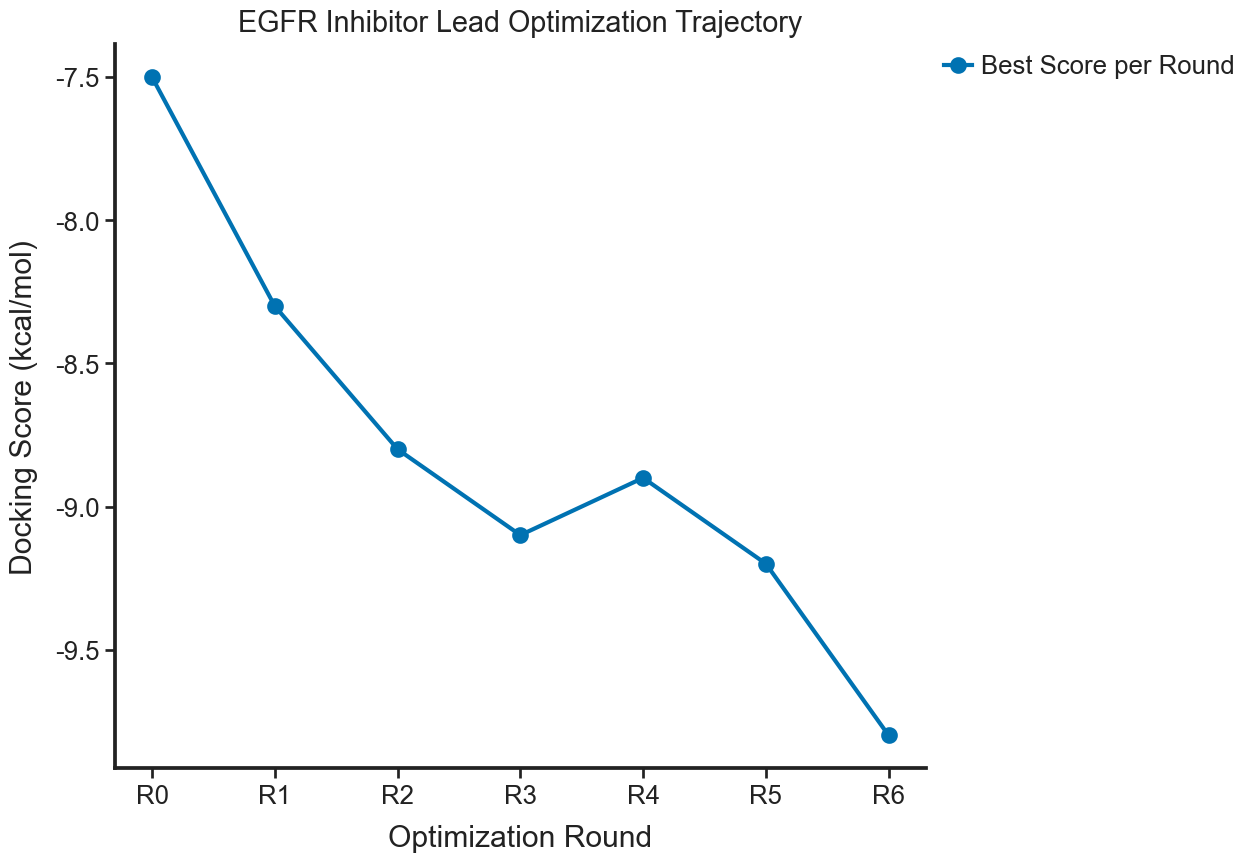
\includegraphics[width=0.48\textwidth]{figures/molclaw_score_trajectory.png}
\hfill
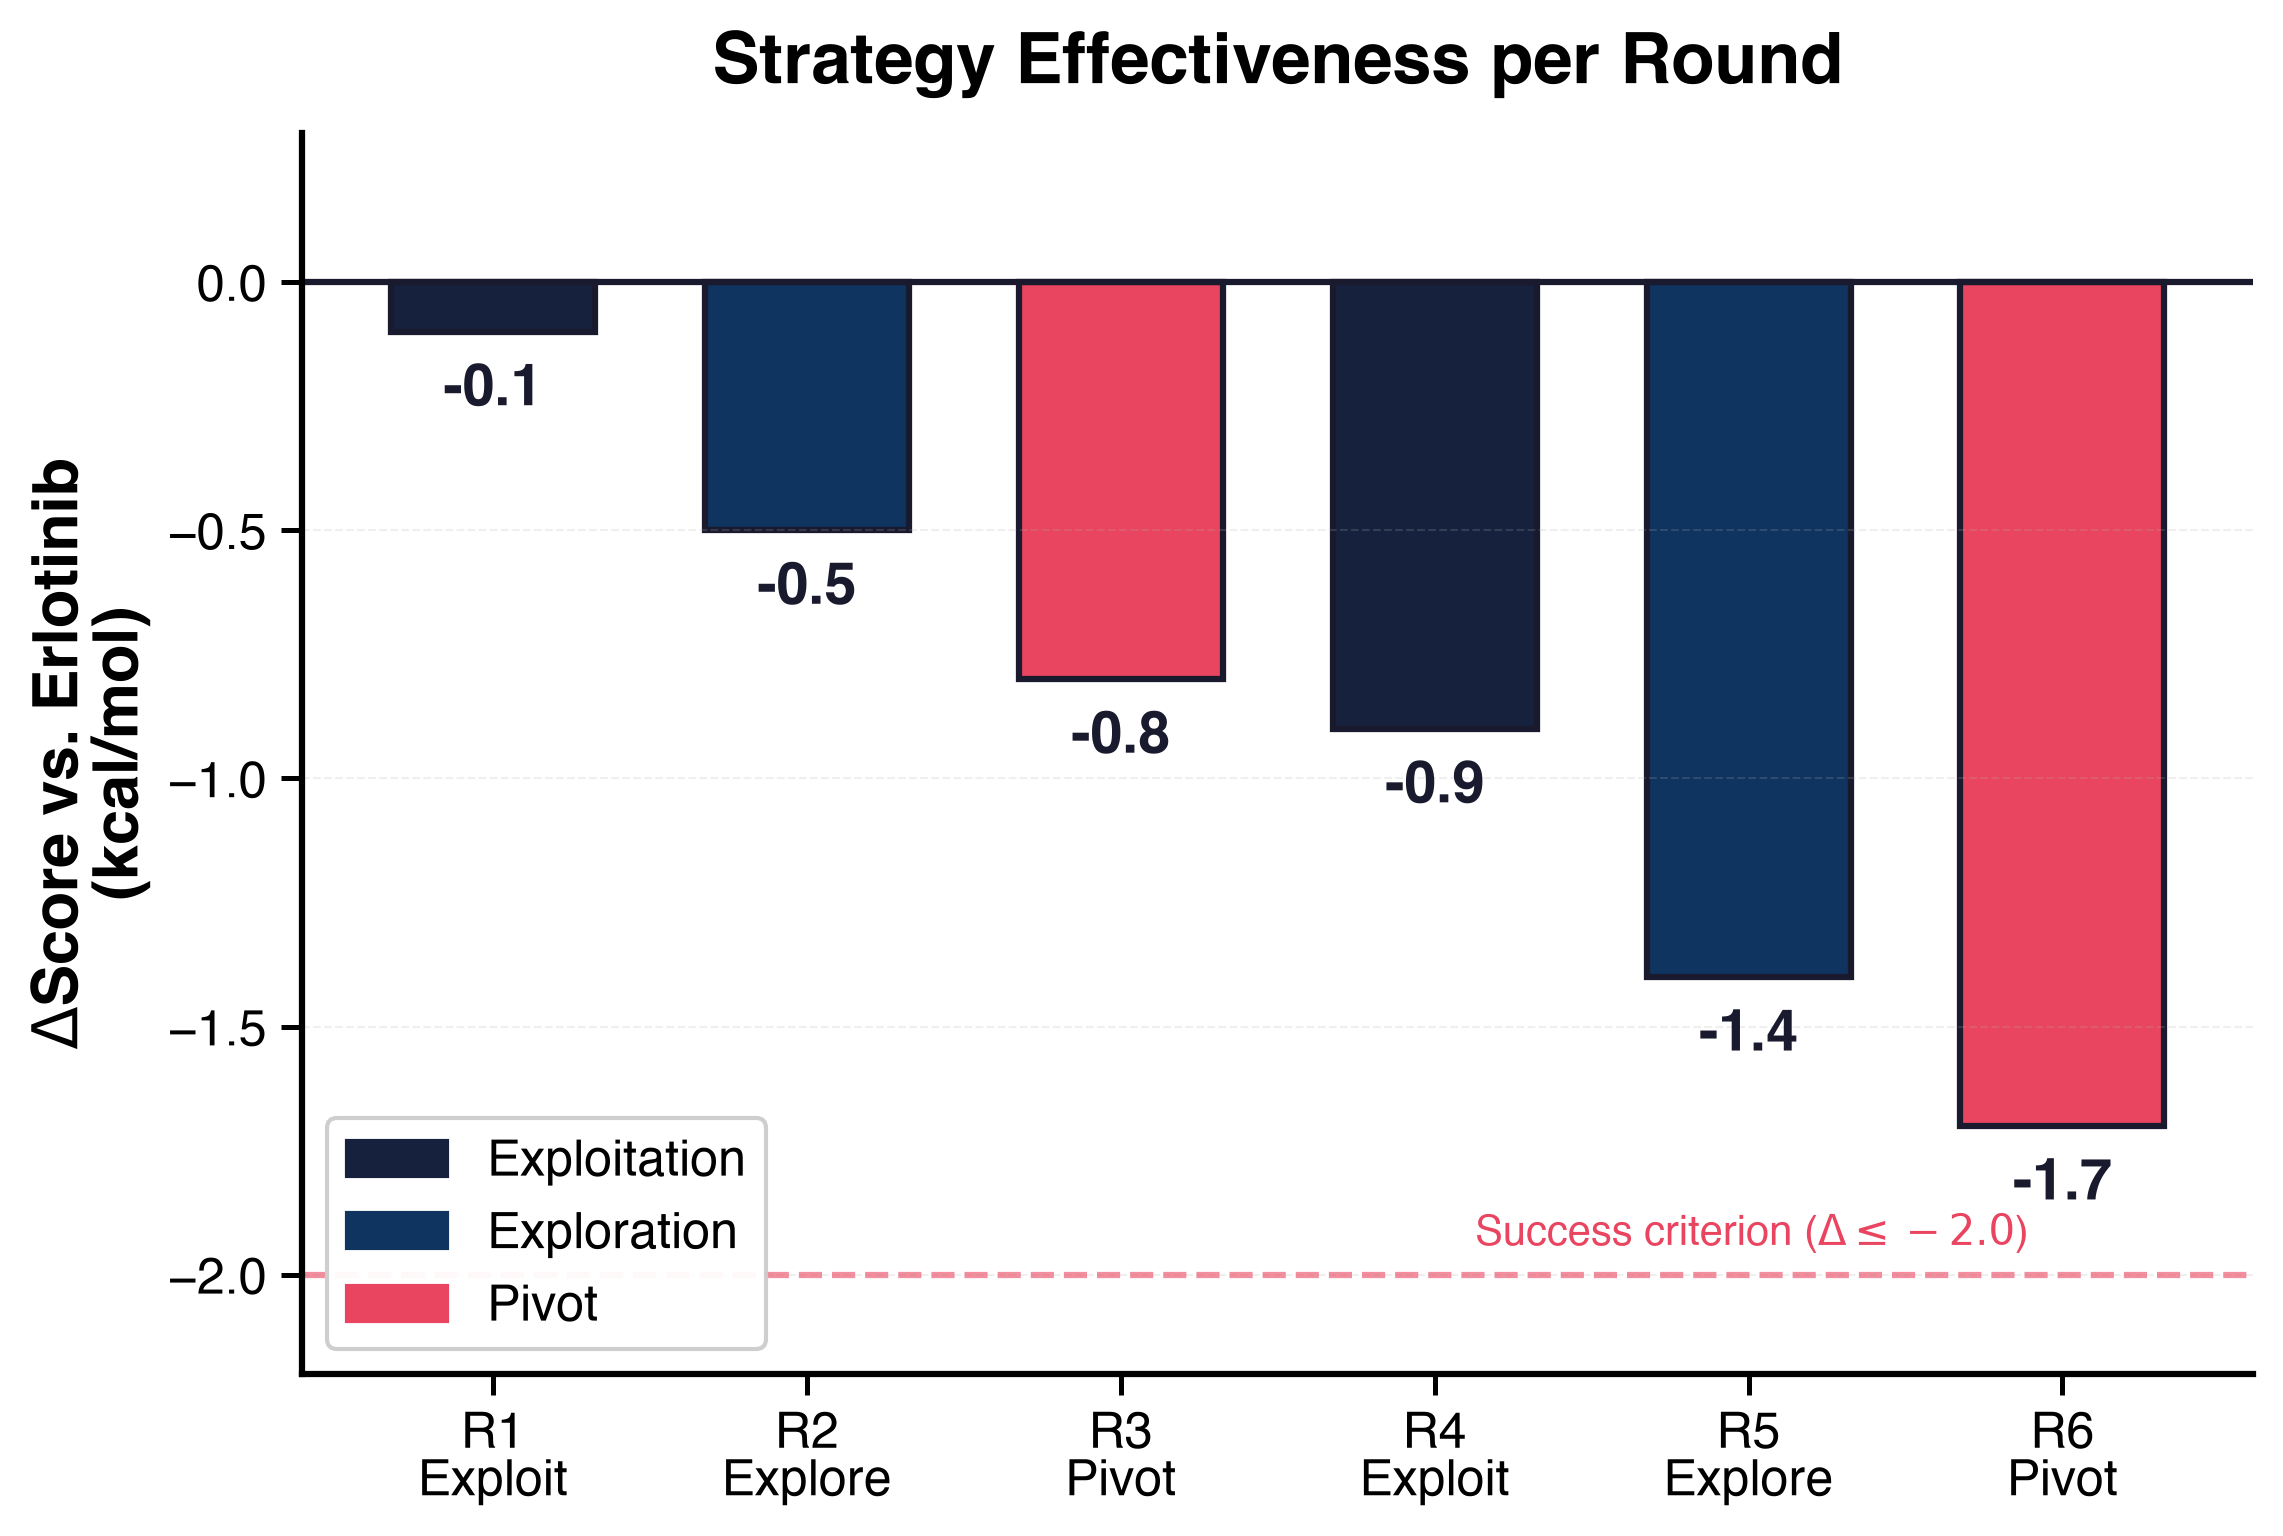
\includegraphics[width=0.48\textwidth]{figures/molclaw_strategy_effectiveness.png}
\caption{(Left) Docking score trajectory across six optimization rounds, showing progressive convergence from $-7.5$ to $-9.8$~kcal/mol. (Right) Strategy effectiveness measured as $\Delta$Score contribution per round, comparing exploration, exploitation, and pivot strategies.}
\label{fig:molclaw-trajectory}
\end{figure}

\textit{Limitations:} The optimized candidates are computational hypotheses; binding affinity, selectivity against off-target kinases, metabolic stability, and synthetic feasibility require orthogonal experimental validation (kinase assays, cellular IC\textsubscript{50}, microsomal stability, and chemical synthesis). QuickVina2-GPU docking scores exhibited 0.9~kcal/mol stochastic variance for identical SMILES across independent runs (EGFR\_R5\_04: $-9.2$ vs.\ EGFR\_R6\_01: $-8.3$), underscoring the need for multiple docking replicates with consensus scoring in production settings. The optimization was constrained to a single scaffold (4-anilinoquinazoline); multi-scaffold exploration, full ADMET profiling, and prospective synthesis with experimental feedback remain future work. The complete run manifest, candidate registry, round-by-round trajectories, and tool evidence are preserved at \url{https://github.com/AGI4Sci/molclaw} for independent review.

\subsection{Computer Use: Genome-to-BGC Discovery and Prioritization}

\textit{[Validated Prototype]} Natural-product discovery from microbial and fungal genomes remains fragmented across bioinformatics tools, databases, and manual interpretation. SciForge's Computer Use harness integrates these stages into a single auditable genome-to-BGC workflow. A researcher provides one or more genome sequences (FASTA, GenBank, or accession ID), and SciForge coordinates the end-to-end pipeline: (1)~genome intake with provenance recording; (2)~antiSMASH-based BGC region discovery; (3)~MIBiG reference matching for known-cluster dereplication; (4)~BiG-SCAPE gene-cluster-family construction with network-neighbor context; (5)~Candidate BGC Card generation unifying genomic, family, dereplication, mechanism, and actionability evidence; (6)~multi-Agent scientific analysis covering mining, dereplication, network interpretation, mechanism reasoning, experiment design, and independent review; and (7)~versioned prioritization separating deterministic card features from Agent interpretation.

We validated this workflow on a four-dataset benchmark comprising 430 antiSMASH-predicted BGC regions, each producing a structured Candidate BGC Card. BiG-SCAPE assigned 408 cards (94.9\%) to gene-cluster families, and MIBiG v4.0 provided dereplication references. A frozen evaluation rubric (v0.1) grounded in the antiSMASH, BiG-SCAPE, MIBiG, and fungal secondary-metabolism literature was applied across all cards, yielding a mean score of 2.750, median 2.740, and range 1.333--3.691 on a nominal 0--5 scale. The rubric stratified cards into four verdict groups: 23 \texttt{priority\_for\_followup}, 111 \texttt{promising\_but\_needs\_dereplication}, 211 \texttt{retain\_for\_context}, and 85 \texttt{low\_priority\_until\_more\_evidence}. Each prioritization cites card evidence fields and separates tool-derived observations from Agent interpretation. The complete run manifest, score table, rubric version, and evidence-card archive are preserved at \url{https://github.com/wenne-kwj/scenario-bgc-genome-discovery} for independent review and manuscript drafting.

\textit{Limitations:} The 23 priority candidates are computational hypotheses; molecular identity, bioactivity, and biological mechanism require orthogonal structural, metabolomic, genetic, or wet-lab validation. The rubric weights and thresholds have not been prospectively calibrated against expert consensus or experimental outcomes. The study was conducted on a fixed benchmark; prospective submission of new genomes with iterative experimental feedback remains future work.

\begin{figure}[ht!]
\centering
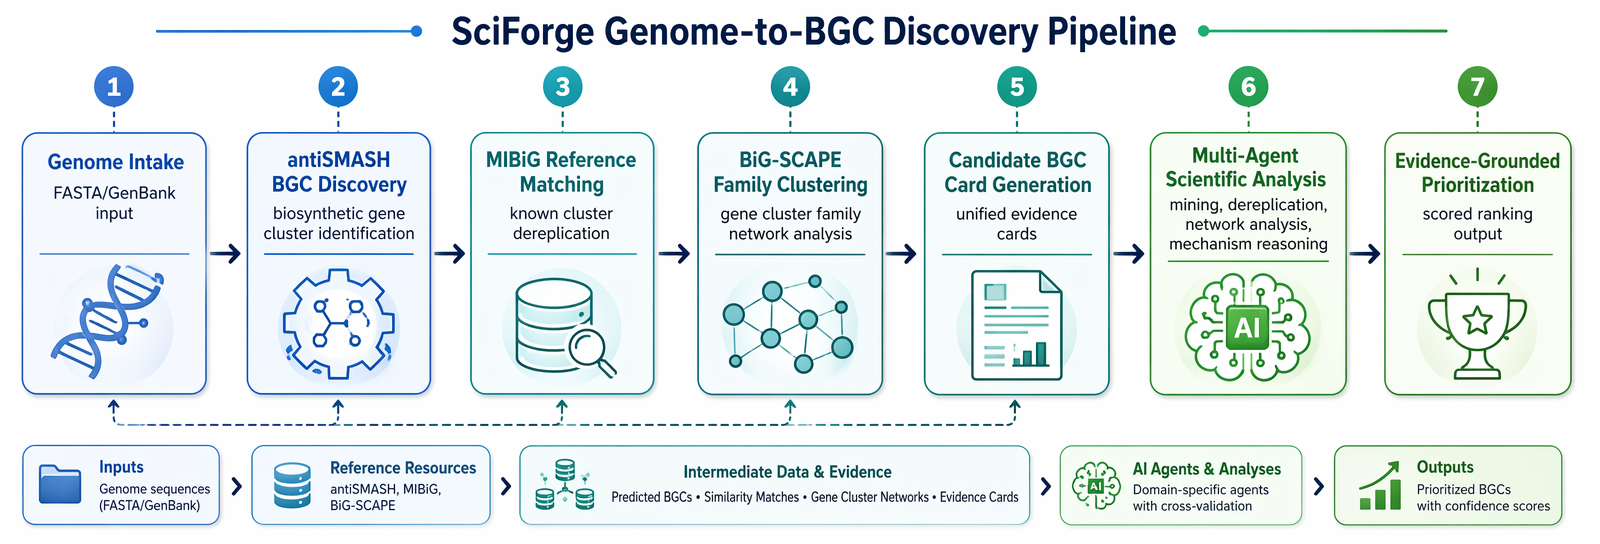
\includegraphics[width=0.95\textwidth]{figures/bgc-workflow.png}
\caption{SciForge Genome-to-BGC Discovery pipeline. The workflow integrates genome intake, antiSMASH BGC discovery, MIBiG reference matching, BiG-SCAPE family clustering, Candidate BGC Card generation, multi-Agent scientific analysis, and evidence-grounded prioritization into a single auditable research record.}
\label{fig:bgc-workflow}
\end{figure}

\FloatBarrier
% ============================================================
\section{Evaluation}
% ============================================================

SciForge is designed as a research infrastructure platform, not as a single-task algorithm whose performance is measured by a scalar metric. We therefore frame evaluation around four questions that are relevant for a goal-oriented, multimodal, auditable, and collaborative research workbench, and identify what the current codebase and public scenario artifacts can support versus what requires future systematic evaluation.

\subsection{Evaluation Questions and Criteria}

\begin{enumerate}
    \item \textbf{Modality Routing Coverage.} Does the Scientific Model Router correctly detect modality, select the configured translator, and attach provenance-annotated observations? \textit{Current evidence:} four translator paths (Esm2Text, Prot2Text, BioT5, C2S) are implemented with unit-level integration in the codebase; Cell2Sentence (C2S) provides translate-then-reason for single-cell transcriptomics (.h5ad files), the same ingress pattern as the other three translators; VCF/BED/GFF/MGF are unsupported and fail closed. \textit{Future:} systematic coverage benchmarks across standard bioinformatics file corpora, false-positive/negative routing rates, and comparison against manual modality annotation.
    \item \textbf{Provenance Completeness.} Does the Evidence DAG capture artifact identity, source anchors, software versions, parameters, and execution traces? \textit{Current evidence:} PROV-JSON schemas and audit-sidecar contracts are present in the codebase; scenario-01, MCFST, and reviewer/rebuttal repositories archive selected workflow artifacts. Commit count alone does not constitute provenance or scientific validity evidence. \textit{Future:} completeness audits against a ground-truth provenance corpus, measurement of missing-link rates under long-running agentic loops, and comparison against manual lab-notebook logging.
    \item \textbf{Reproducibility.} Can a third party re-execute a recorded workflow from versioned artifacts and scripts? \textit{Current evidence:} the cell-atlas pipeline is an illustrative specification (no execution artifacts are available); scenario-01 and MCFST repositories archive outputs but have not undergone third-party re-execution. \textit{Future:} third-party re-execution trials with environment recreation, runtime variability measurement, and comparison against containerized workflow systems.
    \item \textbf{Audit and Decision Governance.} Does the audit layer flag fragile claims, and does the release gate correctly distinguish blocking from non-blocking findings? \textit{Current evidence:} lightweight decision-record contracts and the five-category fragility taxonomy are defined; the reviewer/rebuttal sprint exercises these on a single manuscript as a prototype demonstration, not a validated deployment. \textit{Future:} controlled injection studies with known-weak and known-strong claims, measurement of false-positive and false-negative audit rates, and user studies on decision-making efficiency under audit guidance.
\end{enumerate}

\subsection{Current Evidence Scope and Future Evaluation}

The four evaluation criteria above are currently supported by (a)~the code-level contracts, schemas, and CI-visible tests present in the SciForge repository; (b)~the scenario-01 research sprint repository (archive available at time of writing); (c)~the MCFST paper reproduction repository; and (d)~the reviewer/rebuttal sprint repository. Together these artifacts constitute existence proofs that selected architectural components are instantiated in running code---they do \emph{not} constitute systematic quantitative evaluation. Existence proofs demonstrate selected components and demonstrations; they are not a substitute for systematic evaluation.

The following evaluation categories are explicitly identified as \textbf{future work}: (i)~baseline comparisons against alternative scientific workbench systems or manual workflows; (ii)~ablation studies that isolate the contribution of individual components (e.g., translator routing, Evidence DAG, audit layer); (iii)~inter-annotator agreement or expert-consensus studies on audit findings and evidence quality; (iv)~time-to-completion or researcher-efficiency studies under controlled protocols; (v)~scalability benchmarks under long-running multi-day agentic loops. We encourage the community to contribute protocols, benchmark datasets, and reproducibility studies that exercise these dimensions on the SciForge platform.


\section{Discussion}
% ============================================================

\subsection{Design Trade-offs}

SciForge deliberately favors local control, inspectable state, and modular capability boundaries over a single fully managed cloud service. This improves privacy, deployment flexibility, and laboratory control, but it also requires careful configuration of local models, worker services, scientific connectors, and storage. The same trade-off appears in the Scientific Model Router: domain expert translation improves modality handling and evidence quality, but expert coverage depends on the configured translators and available compute.

The governance layer introduces another trade-off. Recording provenance, claim--evidence links, audit findings, approvals, and artifact review history can make scientific work more auditable, but excessive synchronous gating would slow agent exploration and burden users. SciForge therefore builds the Evidence DAG and runs lightweight audits after completed work or on explicit user request. The Project DAG exposes candidate/certified release records and blocking gate semantics; only product actions explicitly integrated with that API are currently gated.

\subsection{Limitations and Future Work}

The current implementation has several concrete limitations. \textbf{Ingress scope:} end-to-end file ingress is restricted to four modality classes (protein, protein\_structure, molecule, single-cell); Cell2Sentence (C2S) provides translate-then-reason for single-cell transcriptomics (.h5ad files), the same ingress pattern as the other three translators; VCF, BED, GFF, and MGF are unsupported and fail closed. \textbf{Scientific validation:} translator observations are evidence candidates, not verified scientific facts; no systematic validation against ground-truth annotations has been performed. \textbf{Memory model:} research memory stores scoped free-text records rather than a typed scientific state store; typed goals and decisions belong to the Project DAG. \textbf{Evidence completeness:} the Evidence DAG schema can represent complete provenance but depends on runtime capture; software, parameters, environment, log/output, and seed are not automatically populated. \textbf{IM governance:} IM-based coordination is partially integrated; annotation, task transfer, and DAG-decision approval through chat are not end-to-end validated. \textbf{Evaluation gaps:} no baselines, ablation studies, user studies, or third-party reproductions have been conducted. \textbf{MCFST contract:} the verification contract has unresolved conflicts (pre-selection rule, run-count mismatch) and the 0.05 threshold is post-hoc; formal reproduction requires revision and third-party re-execution. \textbf{Cell-atlas provenance:} the cell-atlas pipeline is a specification without execution artifacts; the heatmap is schematic, and \texttt{case45\_gate.py} has not been exercised. Future work includes expanding scientific modality support to crystal structures, mass spectrometry, cryo-EM, and additional omics formats; implementing baselines and systematic evaluations; strengthening IM governance integration; improving provenance capture automation; and developing pre-registered verification contracts with third-party re-execution protocols.

% ============================================================
\section{Conclusion}
% ============================================================

SciForge presents a research-native AI workbench that brings together local execution, scientific multimodal routing, agent orchestration, workflow automation, research memory, and human-governed review surfaces. Its four design pillars---goal-scoped scientific decision governance, translate-then-reason for multimodal input, evidence governance for auditable traceability, and collaborative team science---are designed so that supported native scientific objects become inspectable evidence candidates, captured claims can be linked to provenance records, and release decisions remain reviewable. By combining a local-first workspace with modular worker services and contextual research capability patterns, SciForge aims to serve as a goal-oriented, multimodal, auditable, and collaborative agent operating environment for everyday scientific discovery.

\clearpage
\begin{appendices}
\renewcommand{\theHtable}{A.\arabic{table}}

\section{Capability Differentiation}

\begin{table}[ht!]
\caption{Capability positioning based on reviewed public materials. Typical-approach entries summarize common documented emphases and do not prove absence of unlisted features.}
\label{tab:capability_differentiation}
\scriptsize
\centering
\setlength{\tabcolsep}{2.5pt}
\renewcommand{\arraystretch}{1.08}
\begin{tabular}{@{}L{2.0cm} L{2.4cm} L{2.8cm} L{3.1cm}@{}}
\toprule
\textbf{Capability} & \textbf{Function} & \textbf{Typical approaches} & \textbf{SciForge differentiation} \\
\midrule
Model Router
& Select the optimal LLM provider and model per request
& Single-provider lock-in or manual model switching
& Provider-agnostic routing across OpenAI, Anthropic, DeepSeek, and local models; cost-aware fallback chains; localizable deployment \\
Scientific Pipeline
& Translate scientific file formats into evidence the agent can reason over
& Raw text input or manual format conversion
& Four domain-expert translators (Esm2Text, Prot2Text, BioT5, Cell2Sentence~(C2S)) covering protein, structure, molecule, and single-cell modalities; unrecognized formats fail closed with diagnostics \\
Agent Runtime
& Execute AI agents with tools, sub-agents, and workspace operations
& Single-session chat without structured delegation
& Multi-backend support (Codex, Claude Code, custom runtimes); sub-agent delegation; MCP worker invocation; long-task recovery \\
Workflow Engine
& Chain research steps into repeatable, scheduled protocols
& Ad-hoc scripts and cron jobs
& DAG-based workflows with code, agent, tool, and approval nodes; schedule and event triggers; integrated with agent runtime \\
Research Memory
& Store and retrieve project knowledge across sessions
& Ephemeral chat history or external document RAG
& Structured Project DAG with confidence-tagged, scoped free-text records; typed goals and decision events persist across sessions \\
Evidence Governance
& Track provenance, audit claims, and govern release decisions
& Outputs detached from data, scripts, and review history
& Thread-scoped Evidence DAGs with automatic provenance capture; deterministic audit runs; goal-scoped release gates \\
Research Capability Patterns
& Define structured human judgment points at research milestones
& Generic chat and file-list views
& Six recurrent interaction patterns (artifact review, approval, visual inspection, etc.) grounded in Evidence DAGs and audit records \\
\bottomrule
\end{tabular}
\end{table}
\clearpage

\end{appendices}

% ============================================================
% Resource
% ============================================================
\section*{Resource}

The SciForge codebase, including the Evidence-DAG audit worker, lightweight decision-record contracts, agentic skills, and scientific model router, is open source and available at:

\vspace{4pt}
\centering
\url{https://github.com/AGI4Sci/SciForge}
\vspace{8pt}

\noindent The MCFST paper reproduction artifacts---including generated code, preprocessed data, prediction outputs, and result figures---are available at:

\vspace{4pt}
\centering
\url{https://github.com/Winshion/sciforge-ai4ai-spacial-trans}
\vspace{8pt}

\noindent Researchers are encouraged to explore both repositories, contribute new skills, workflows, audit rules, and research decision patterns, and develop third-party re-execution protocols for the workflows described in this paper.

% ============================================================
% Bibliography
% ============================================================
\bibliography{sn-bibliography}

\end{document}
